\documentclass{beamer}
\usepackage[utf8]{inputenc}
\usepackage{graphicx}
\usepackage{color}
\usetheme{Madrid}
\usepackage{svg}
\usecolortheme{default}

\title{Master Slave Flip Flop}
\author{Shoumik Saha\inst{1} \and Sanjay Malakar\inst{2} }

\institute % (optional)
{
  \inst{1}%
  1505059
  \and
  \inst{2}%
  1505057
}


\date{July 2018}


\begin{document}

\frame{\titlepage}


%flip flop
\begin{frame}
\frametitle{What is flip flop?}
\begin{itemize}
 \item<1-> A flip flop is an electronic circuit with two stable states that can be used to store binary data.
 \item<2->  Flip-flops are used as data storage elements. It is the basic storage element in sequential logic.
 \item<3->  Flip-flops are fundamental building blocks of digital electronics systems used in computers, communications, and many other types of systems.
\end{itemize}
\end{frame}


%a diff o ff and latch
\begin{frame}
\frametitle{Flip flop v/s Latch}

The basic difference between a latch and a flip-flop is a gating or clocking mechanism. For example, let us talk about SR latch and SR flip-flops.\pause
\begin{columns}
\column{0.5\textwidth}
\begin{figure}[h]
    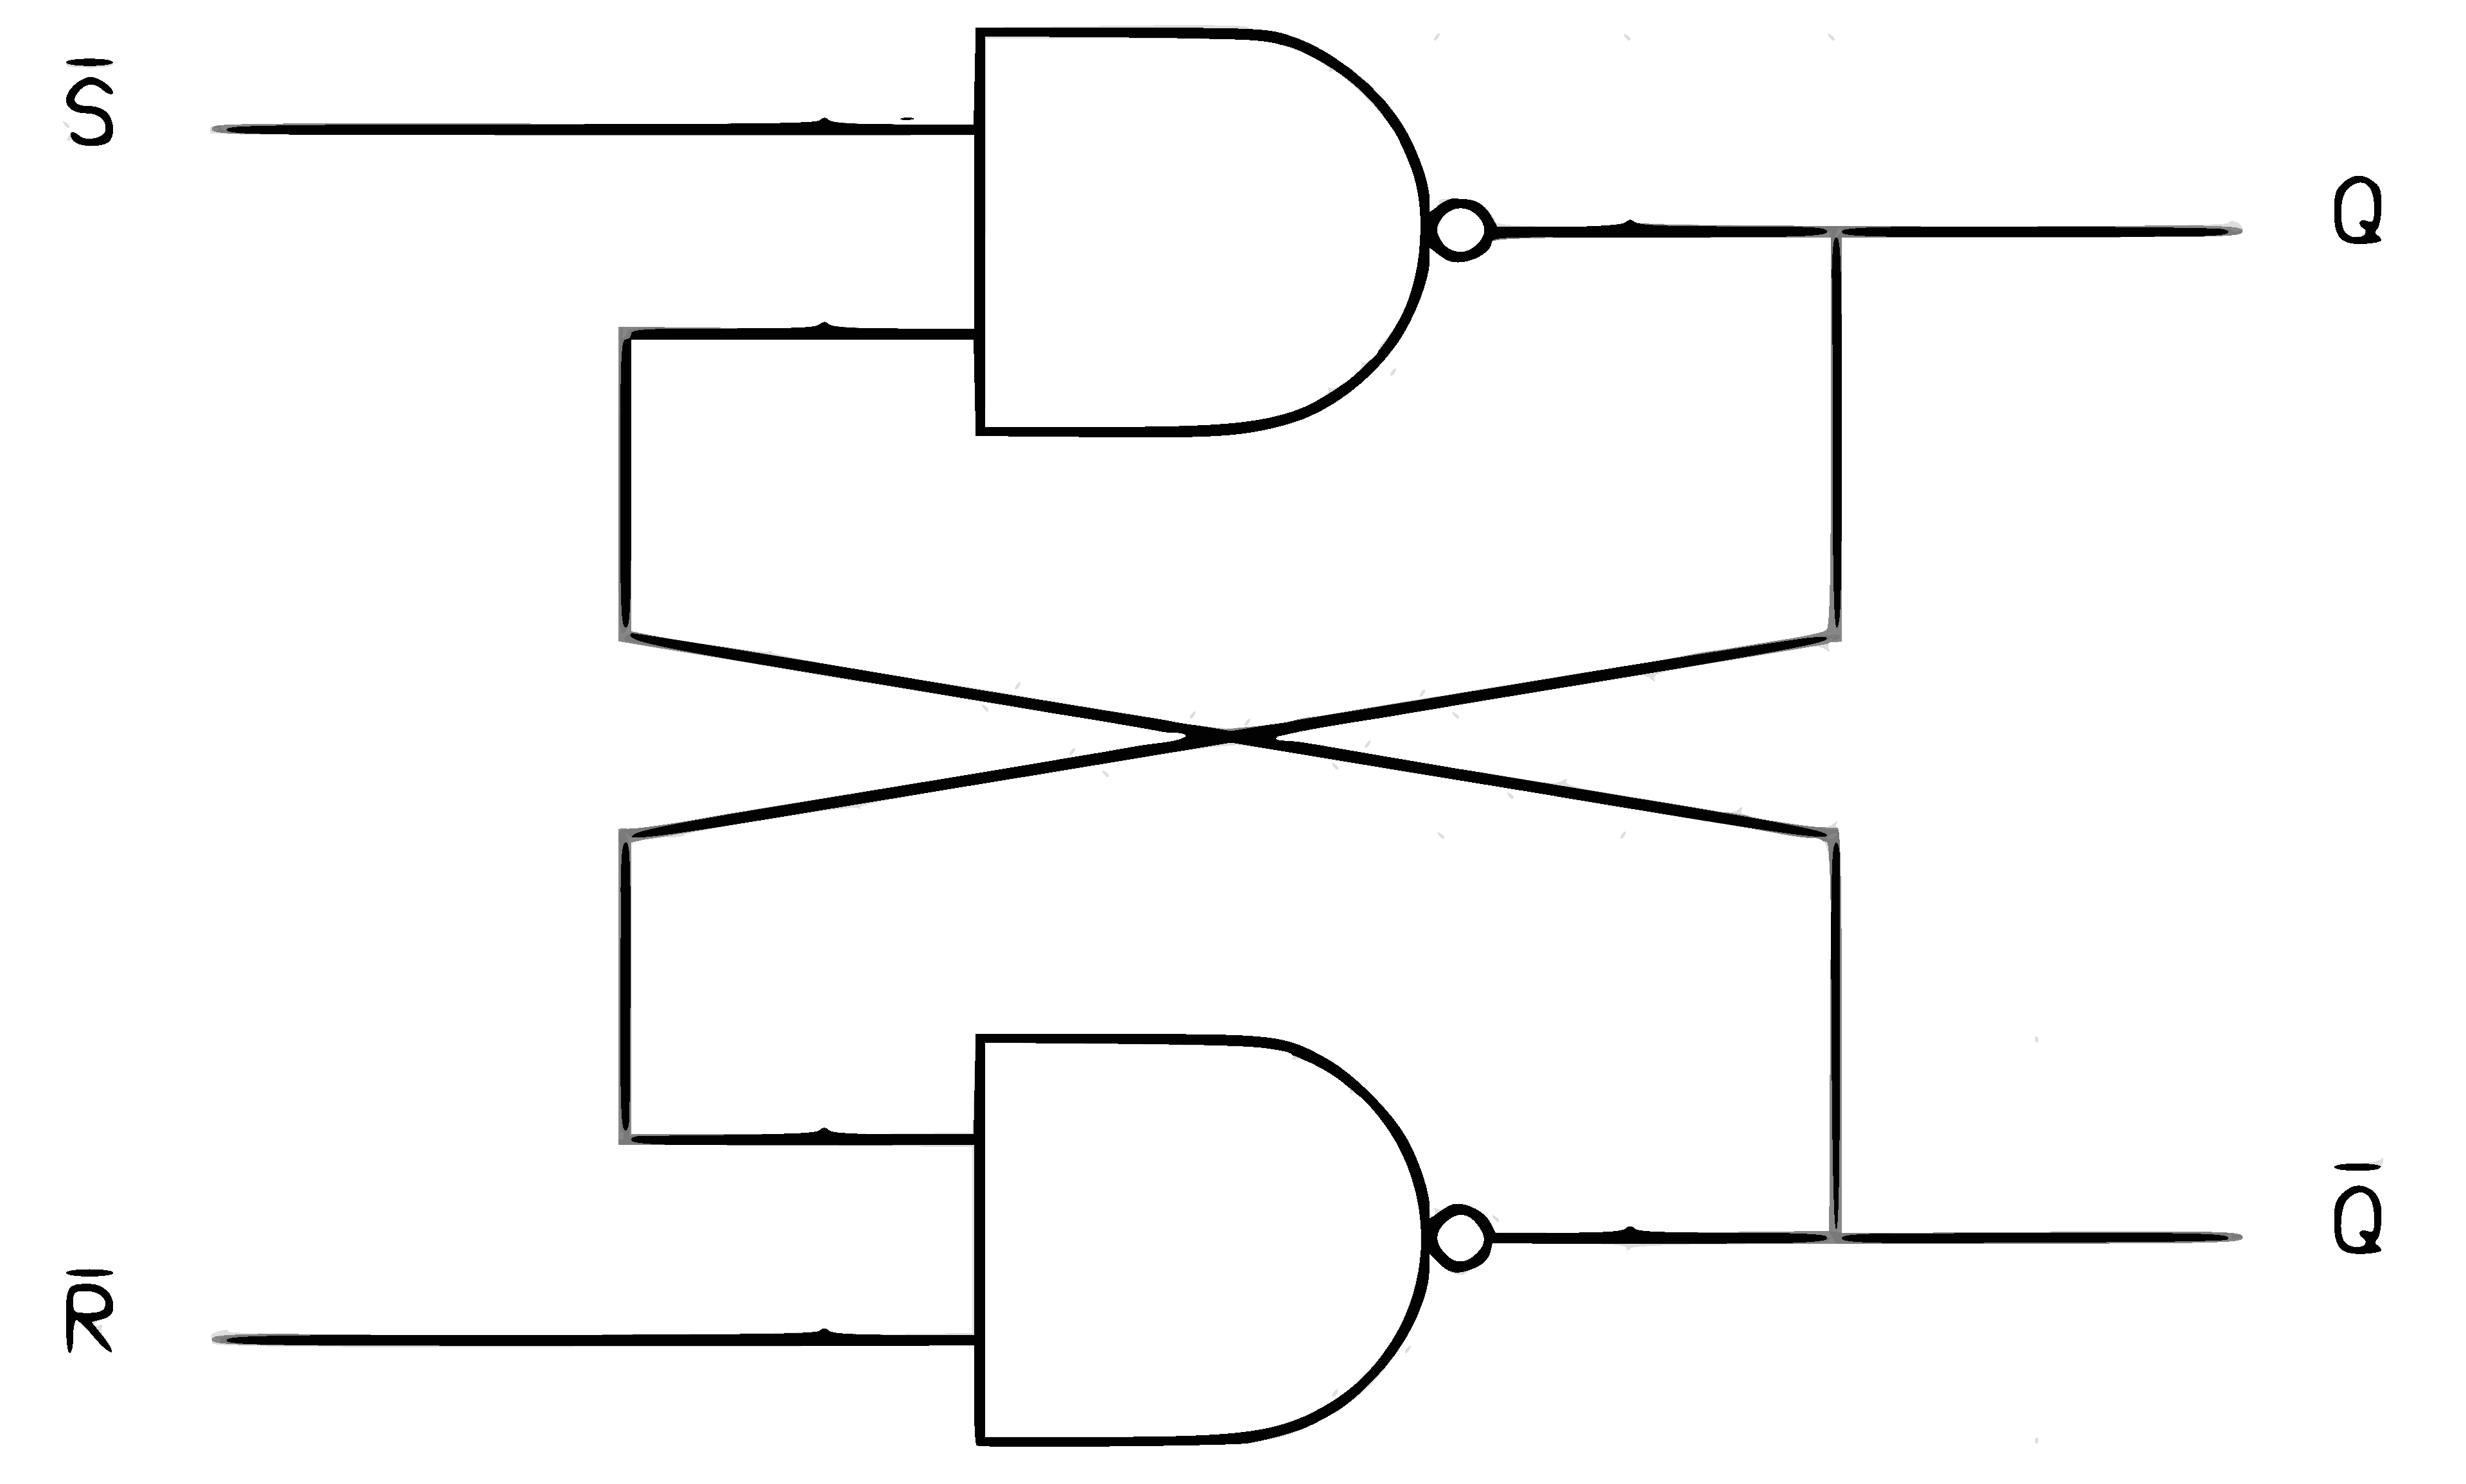
\includegraphics[scale=.033]{srl.png}
    \caption{SR latch}
\end{figure}

 
\column{0.5\textwidth}
\begin{figure}[h]
    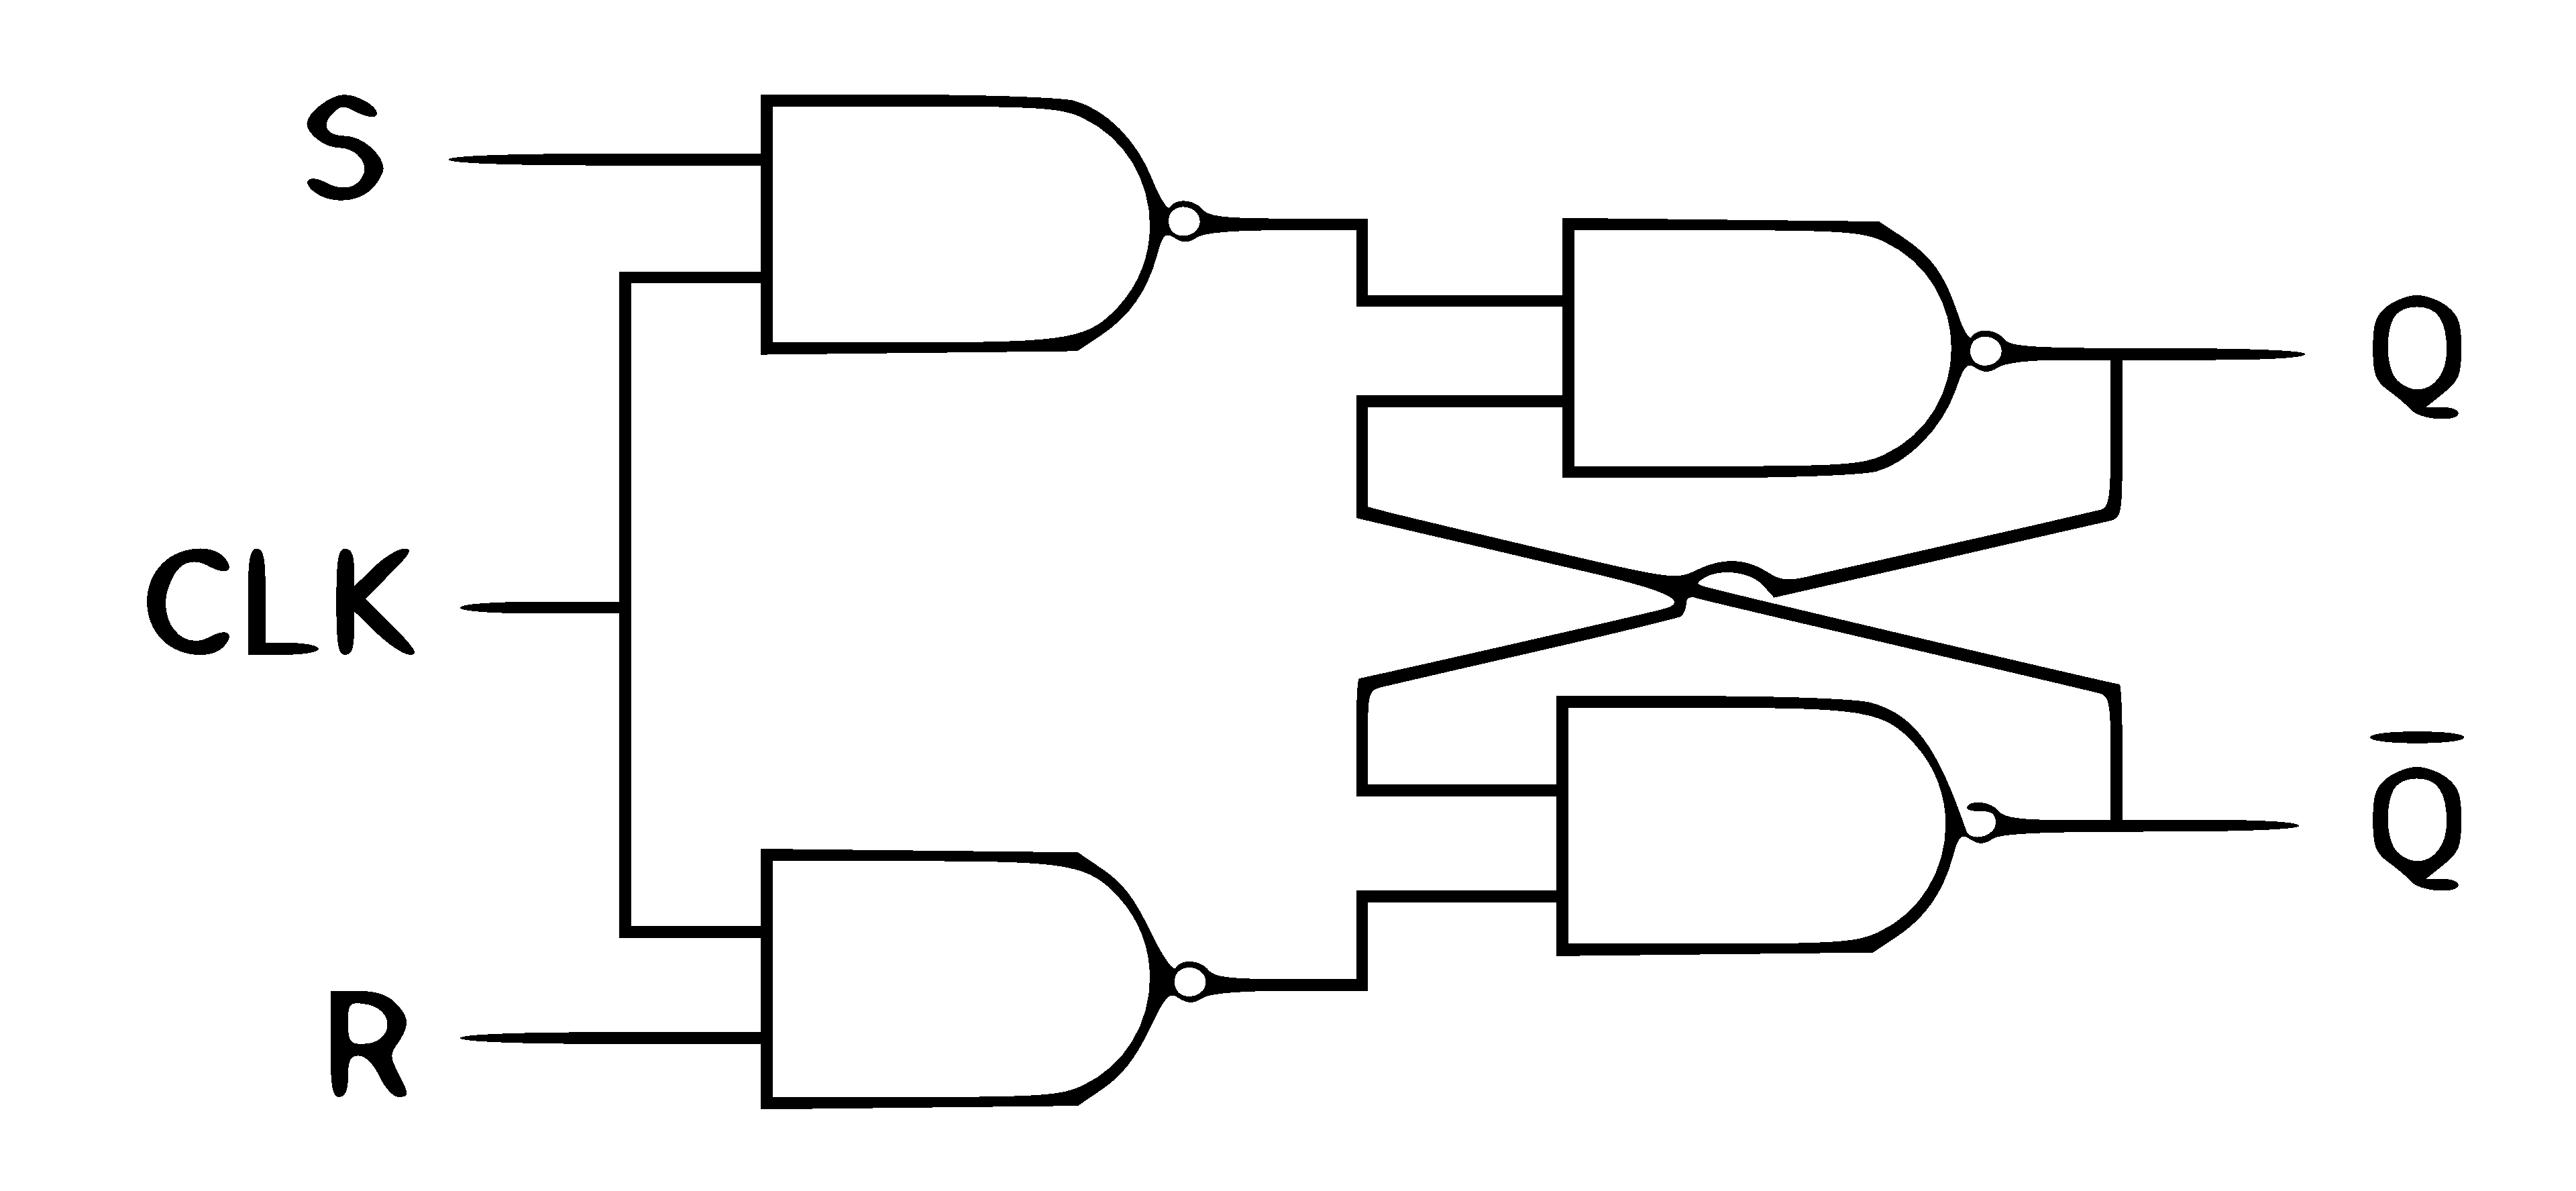
\includegraphics[scale=.033]{srff.png}
    \caption{SR flip flop}
\end{figure}
\end{columns}\pause
A flip flop is synchronous and is also known as gated or clocked SR latch.The output only changes when a active high clock is given.
\end{frame}
\begin{frame}
\frametitle{Flip flop v/s Latch}

The basic difference between a latch and a flip-flop is a gating or clocking mechanism. For example, let us talk about SR latch and SR flip-flops.
\begin{columns}
\column{0.5\textwidth}
\begin{figure}[h]
    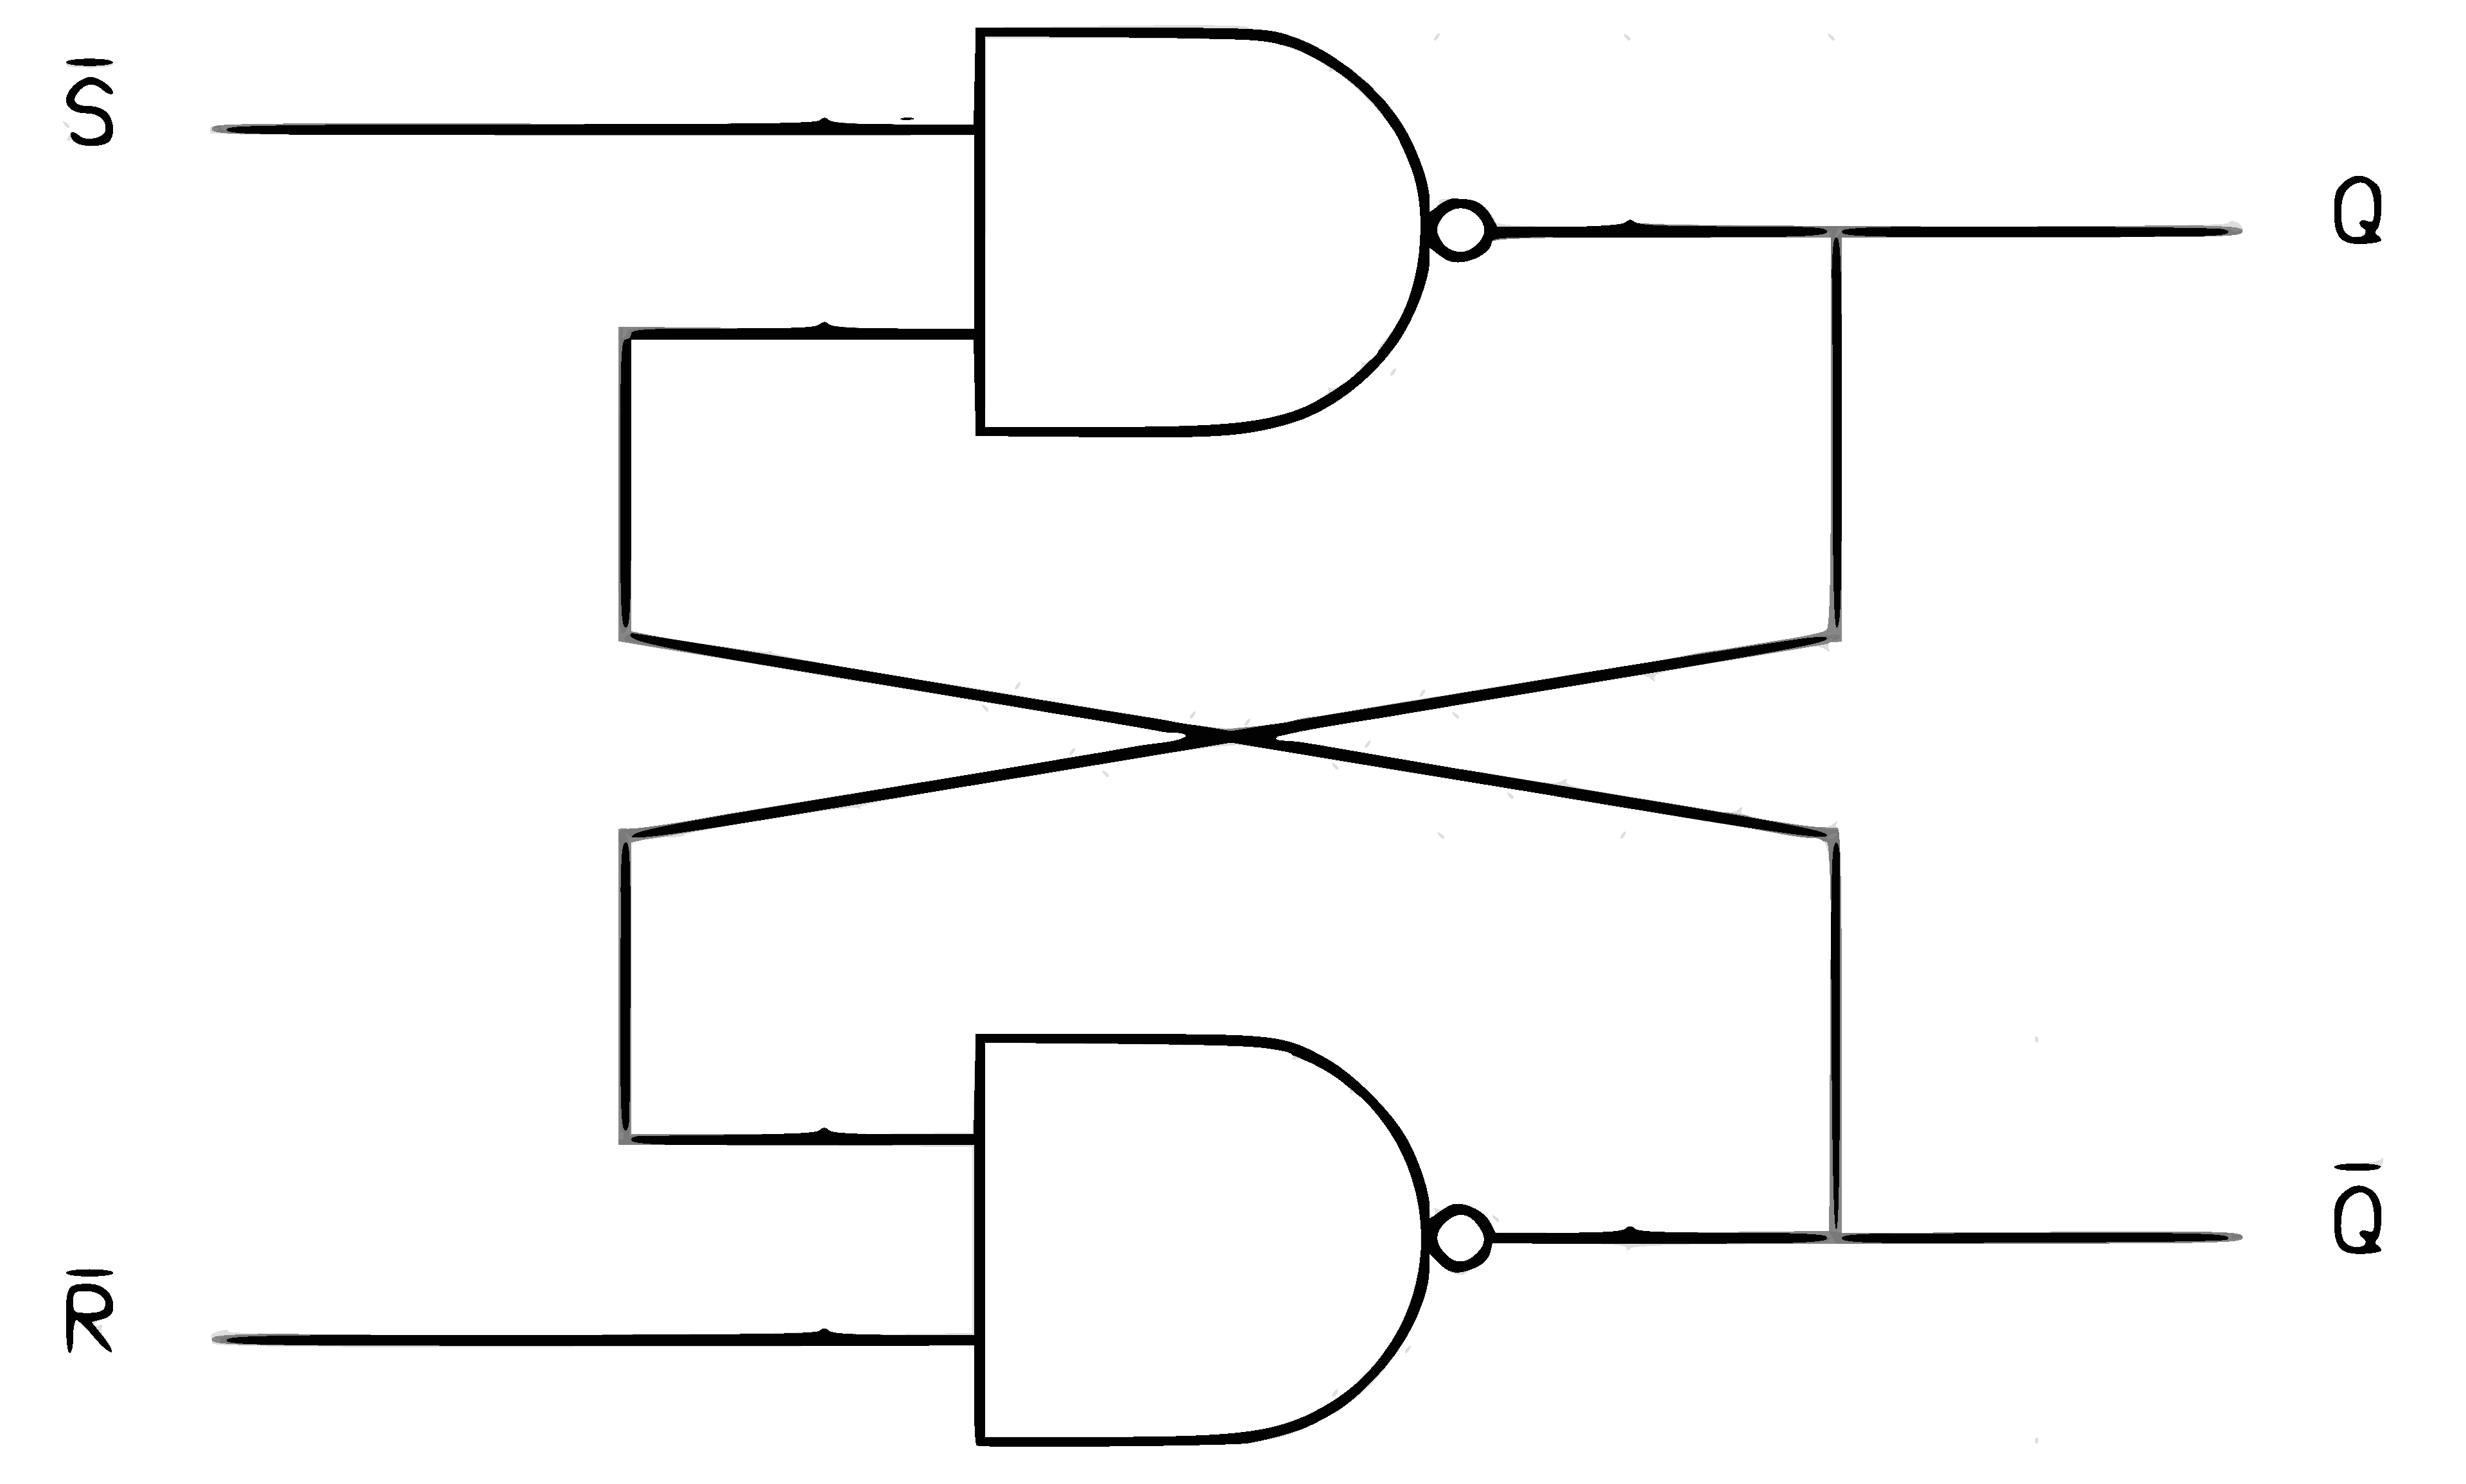
\includegraphics[scale=.033]{srl.png}
    \caption{SR latch}
\end{figure}

 
\column{0.5\textwidth}
\begin{figure}[h]
    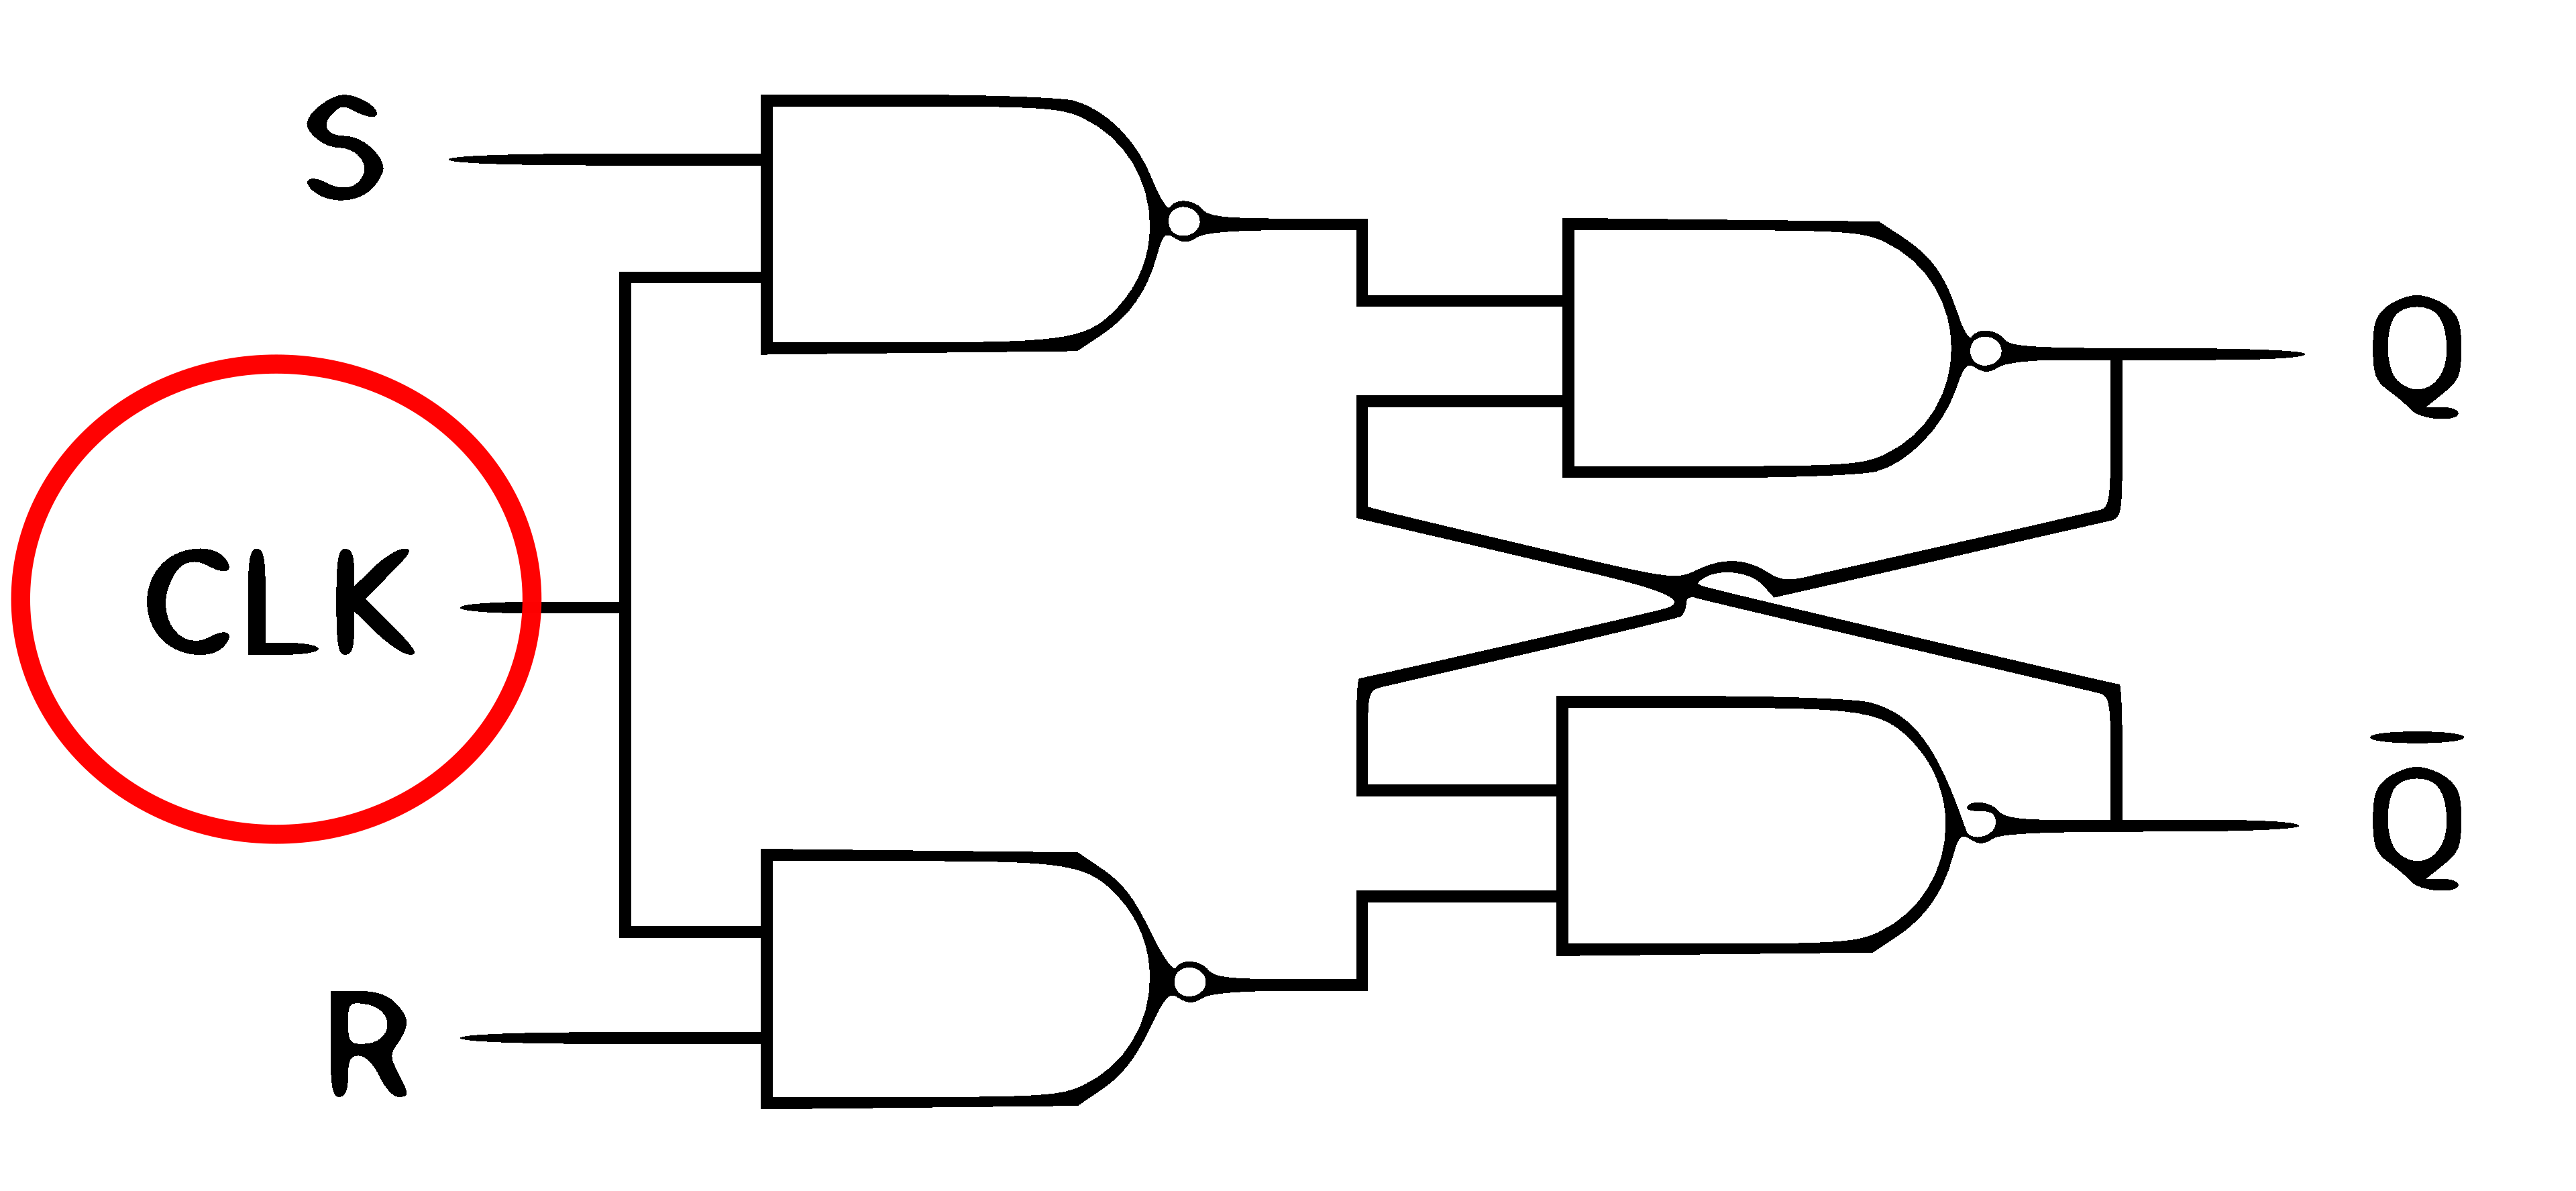
\includegraphics[scale=.033]{srffc.png}
    \caption{SR flip flop}
\end{figure}
\end{columns}
A flip flop is synchronous and is also known as gated or clocked SR latch.The output only changes when a active high clock is given.
\end{frame}


\begin{frame}
\frametitle{Types of flip flop}
\begin{columns}
    \column{0.5\textwidth}
    
    \begin{itemize}
    \item<1-> D Flip Flop\pause
    
    \end{itemize}
    
    \column{0.5\textwidth}
    
    
    
     
    \begin{figure}[H]
        \centering
        
        %\def\svgscale{1}
        \includesvg[width=100pt]{images/D_Flip-flop.svg}
        
        
        \caption{D type Flip Flop}
        \label{fig:my_label}
    \end{figure} \pause
    
    \centering
    \begin{tabular}[H]{ |c|c|c|c| }
    \hline
    Clock & D & Q & \overline Q \\
    \hline
    \hline
    $0$ & $0$ & Q & \overline Q\\  
    $0$ & $1$ & Q & \overline Q\\
    $1$ & $0$ & $0$ & $1$\\
    $1$ & $1$ & $1$ & $0$\\
    \hline
    \end{tabular}
   
    
    
    

\end{columns}
\end{frame}

\begin{frame}

\begin{columns}
    \column{0.5\textwidth}
    
\begin{itemize}
    
    
    \item D Flip Flop 
    \item JK Flip Flop\pause
    
\end{itemize}

    \column{0.5\textwidth}
    \begin{figure}[H]
        \centering
        
        %\def\svgscale{1}
        \includesvg[width=100pt]{images/JK_Flip-flop.svg}
        
        
        \caption{JK type Flip Flop}
        \label{fig:my_label}
    \end{figure}\pause
    
    \begin{figure}[H]
        \centering
        
        %\def\svgscale{1}
        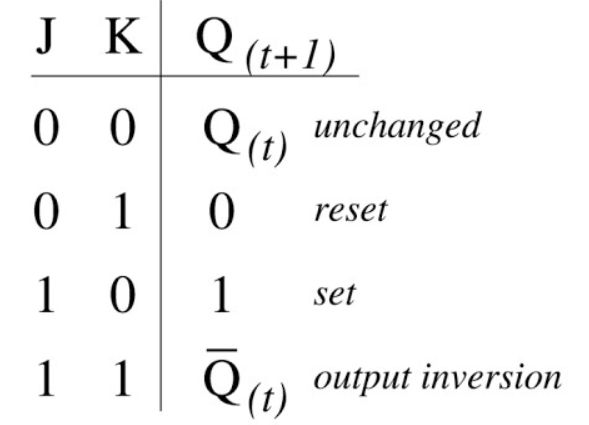
\includegraphics[width=100pt]{name/abc.png}
        
        
        \caption{JK type Flip Flop}
        \label{fig:my_label}
    \end{figure}\pause
    
    
    
    
    \end{columns}
\end{frame}

\begin{frame}

    \begin{columns}
    \column{0.5\textwidth}
    
    \begin{itemize}
    
    
    \item D Flip Flop 
    \item JK Flip Flop
    \item SR Flip Flop\pause
    
\end{itemize}

\column{0.5\textwidth}
    \begin{figure}[H]
        \centering
        
        %\def\svgscale{1}
        \includesvg[width=100pt]{images/SR_Flip-flop.svg}
        
        
        \caption{SR type Flip Flop}
        \label{fig:my_label}
    \end{figure}\pause
    
    \centering
    \begin{tabular}{ |c|c|c|c| }
    \hline
      S & R & Q & \overline Q \\
     \hline
     \hline
     $0$ & $0$ & $0$ & $1$ \\  
     $0$ & $1$ & $0$ & $1$\\
     $1$ & $0$ & $1$ & $0$\\
     $1$ & $1$ & $\infty$ & $\infty$\\
     \hline
    \end{tabular}
    
    
    \end{columns}
\end{frame}

\begin{frame}

    \begin{columns}
    \column{0.5\textwidth}
    
    \begin{itemize}
    
    
    \item D Flip Flop 
    \item JK Flip Flop
    \item SR Flip Flop
    \item T Flip Flop\pause
    
\end{itemize}

\column{0.5\textwidth}
    \begin{figure}[H]
        \centering
        
        %\def\svgscale{1}
        \includesvg[width=100pt]{images/T-Type_Flip-flop.svg}
        
        
        \caption{T type Flip Flop}
        \label{fig:my_label}
    \end{figure}\pause
    
    \begin{figure}[H]
        \centering
        
        %\def\svgscale{1}
        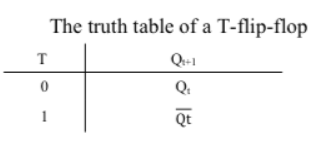
\includegraphics[width=100pt]{name/abc2.png}
        
        

        \label{fig:my_label}
    \end{figure}\pause
    
    
    \end{columns}
\end{frame}

\begin{frame}
\frametitle{Master Slave Flip Flop}
\begin{itemize}
 \item<1-> Master Slave flip flop are the cascaded combination of two flip-flops among which the first is designated as master flip-flop while the next is called slave flip-flop (Figure 1).
 \item<2-> The master flip-flop is triggered by the external clock pulse train while the slave is activated at its inversion i.e. if the master is positive edge-triggered, then the slave is negative-edge triggered and vice-versa.
 \item<3-> This means that the data enters into the flip-flop at leading/trailing edge of the clock pulse while it is obtained at the output pins during trailing/leading edge of the clock pulse. Hence a master-slave flip-flop completes its operation only after the appearance of one full clock pulse for which they are also known as \alert{pulse-triggered} flip-flops.
 \end{itemize}

\end{frame}

\begin{frame}
\frametitle{Master slave implementation using different flip flops}
\begin{figure}[h]
    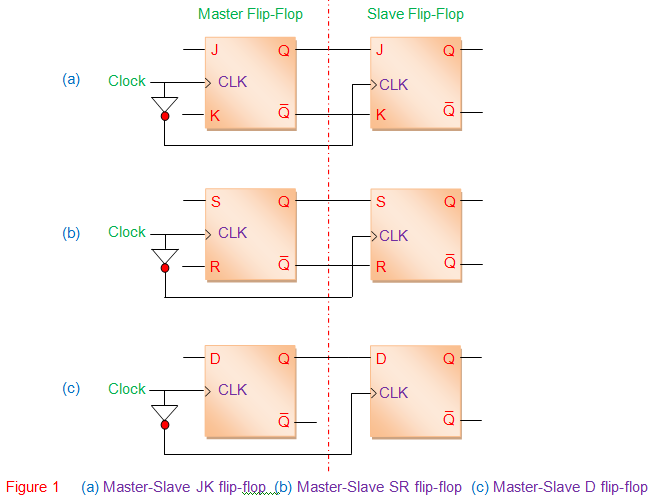
\includegraphics[scale=.45]{msffs.PNG}
\end{figure}
\end{frame}


\begin{frame}{Implementation with gates}
    We will learn how to implement Master Slave D flip flop with NAND gates.\newline \pause
    Let's construct the first part of our Master Slave flip flop.\pause
    \begin{figure}[H]
        \centering
        
        %\def\svgscale{1}
        \includesvg[scale=.7]{images/masterNandsvg.svg}
        
        
        %\caption{T type Flip Flop}
        \label{fig:my_label}
    \end{figure}
    
\end{frame}

\begin{frame}{Implementation with gates}
   
    Let's construct the second part of our Master Slave flip flop.\pause
    \begin{figure}[H]
        \centering
        
        %\def\svgscale{1}
        \includesvg[width=\textwidth,height=500pt]{images/masterSlaveNandsvg.svg}
        
        
        %\caption{T type Flip Flop}
        \label{fig:my_label}
    \end{figure}
    
\end{frame}

\begin{frame}{Implementation with gates}
   
    
    \begin{figure}[H]
        \centering
        
        %\def\svgscale{1}
        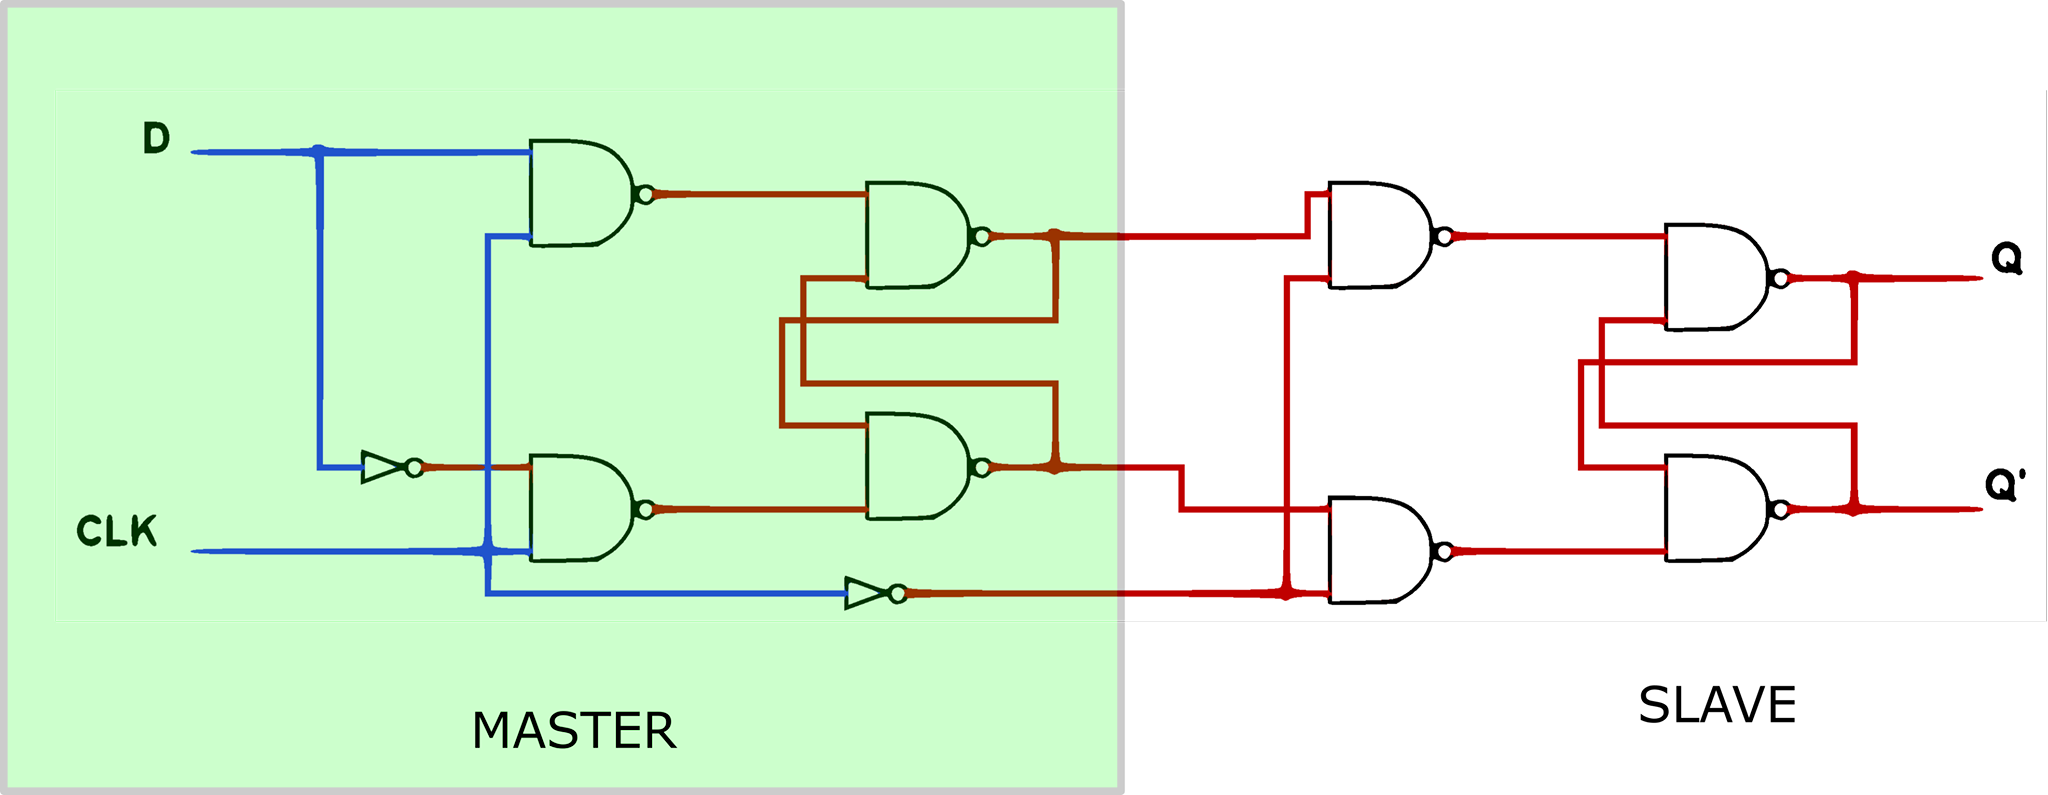
\includegraphics[scale=.15]{images/masterNandsvgBlocked.png}
        
        
        %\caption{T type Flip Flop}
        \label{fig:my_label}
    \end{figure}
    
\end{frame}

\begin{frame}{Implementation with gates}
   
    
    \begin{figure}[H]
        \centering
        
        %\def\svgscale{1}
        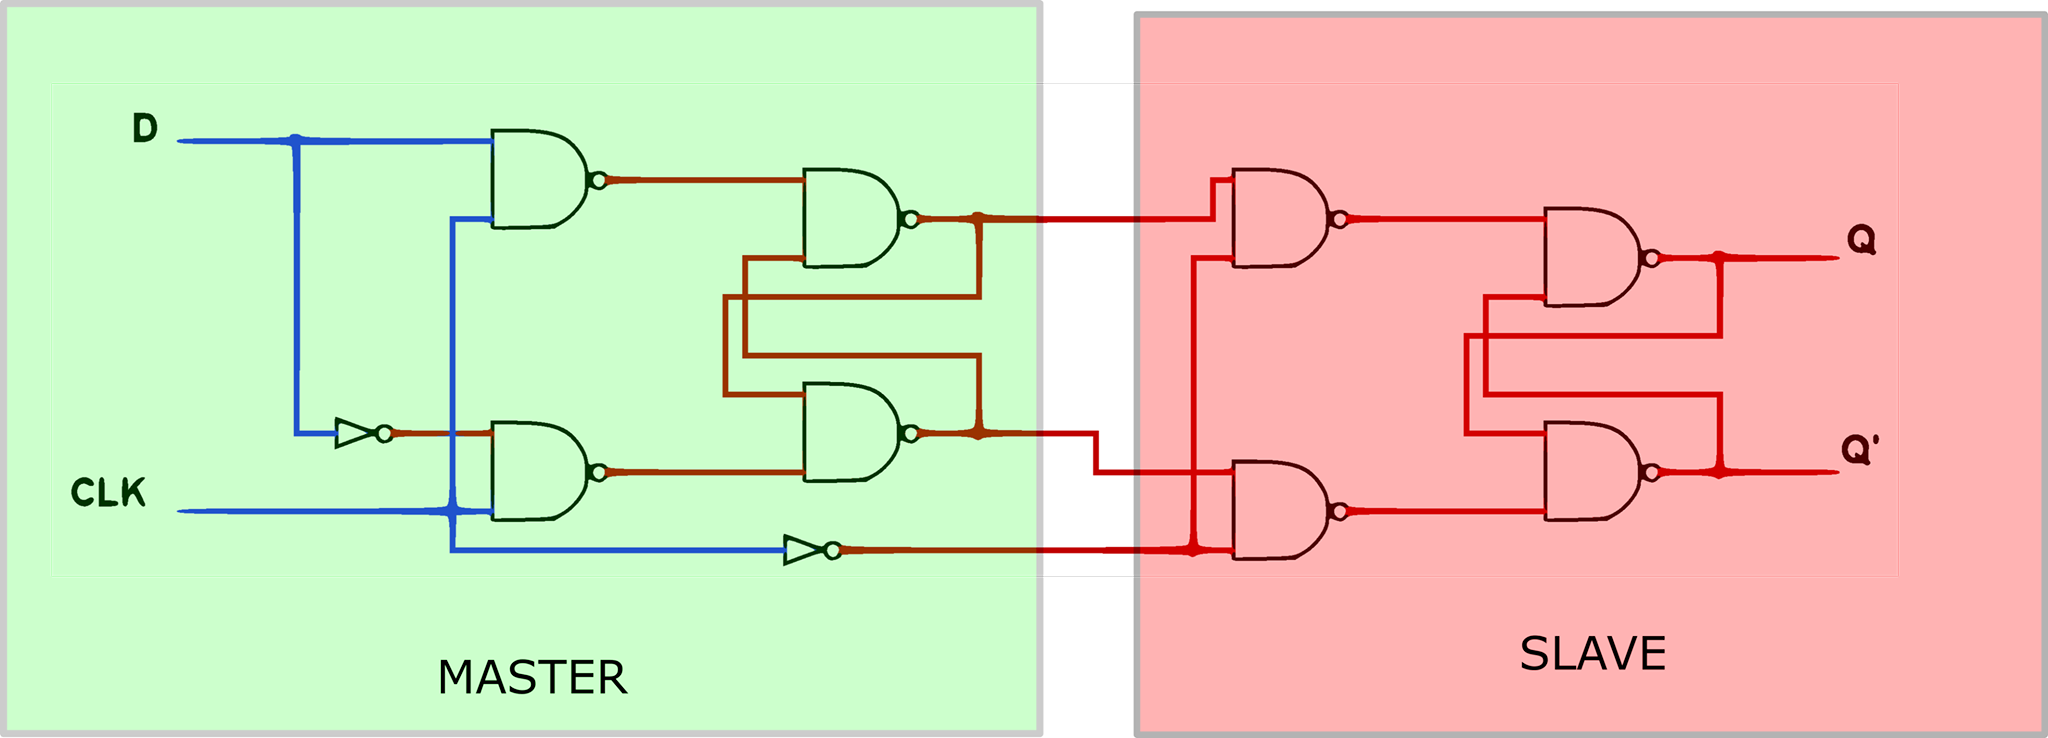
\includegraphics[scale=.15]{images/masterSlaveNandBlocked.png}
        
        
        %\caption{T type Flip Flop}
        \label{fig:my_label}
    \end{figure}
    
\end{frame}


\begin{frame}{Implementation with gates}
    \alert{What should we add to Preset and Clear?}\pause
    
    
    \begin{figure}[H]
        \centering
        
        %\def\svgscale{1}
        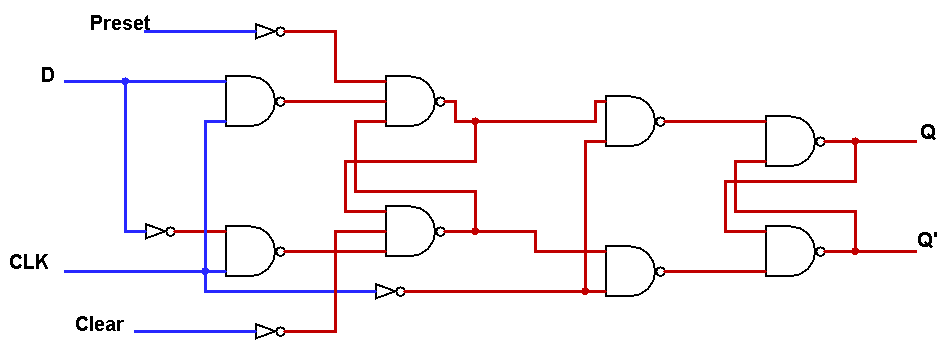
\includegraphics[scale=.35]{images/withPresetClear.png}
        
        
        %\caption{T type Flip Flop}
        \label{fig:my_label}
    \end{figure}
    
\end{frame}

\begin{frame}
\frametitle{Simulation of Master Slave D flip flop}
\begin{figure}[h]
    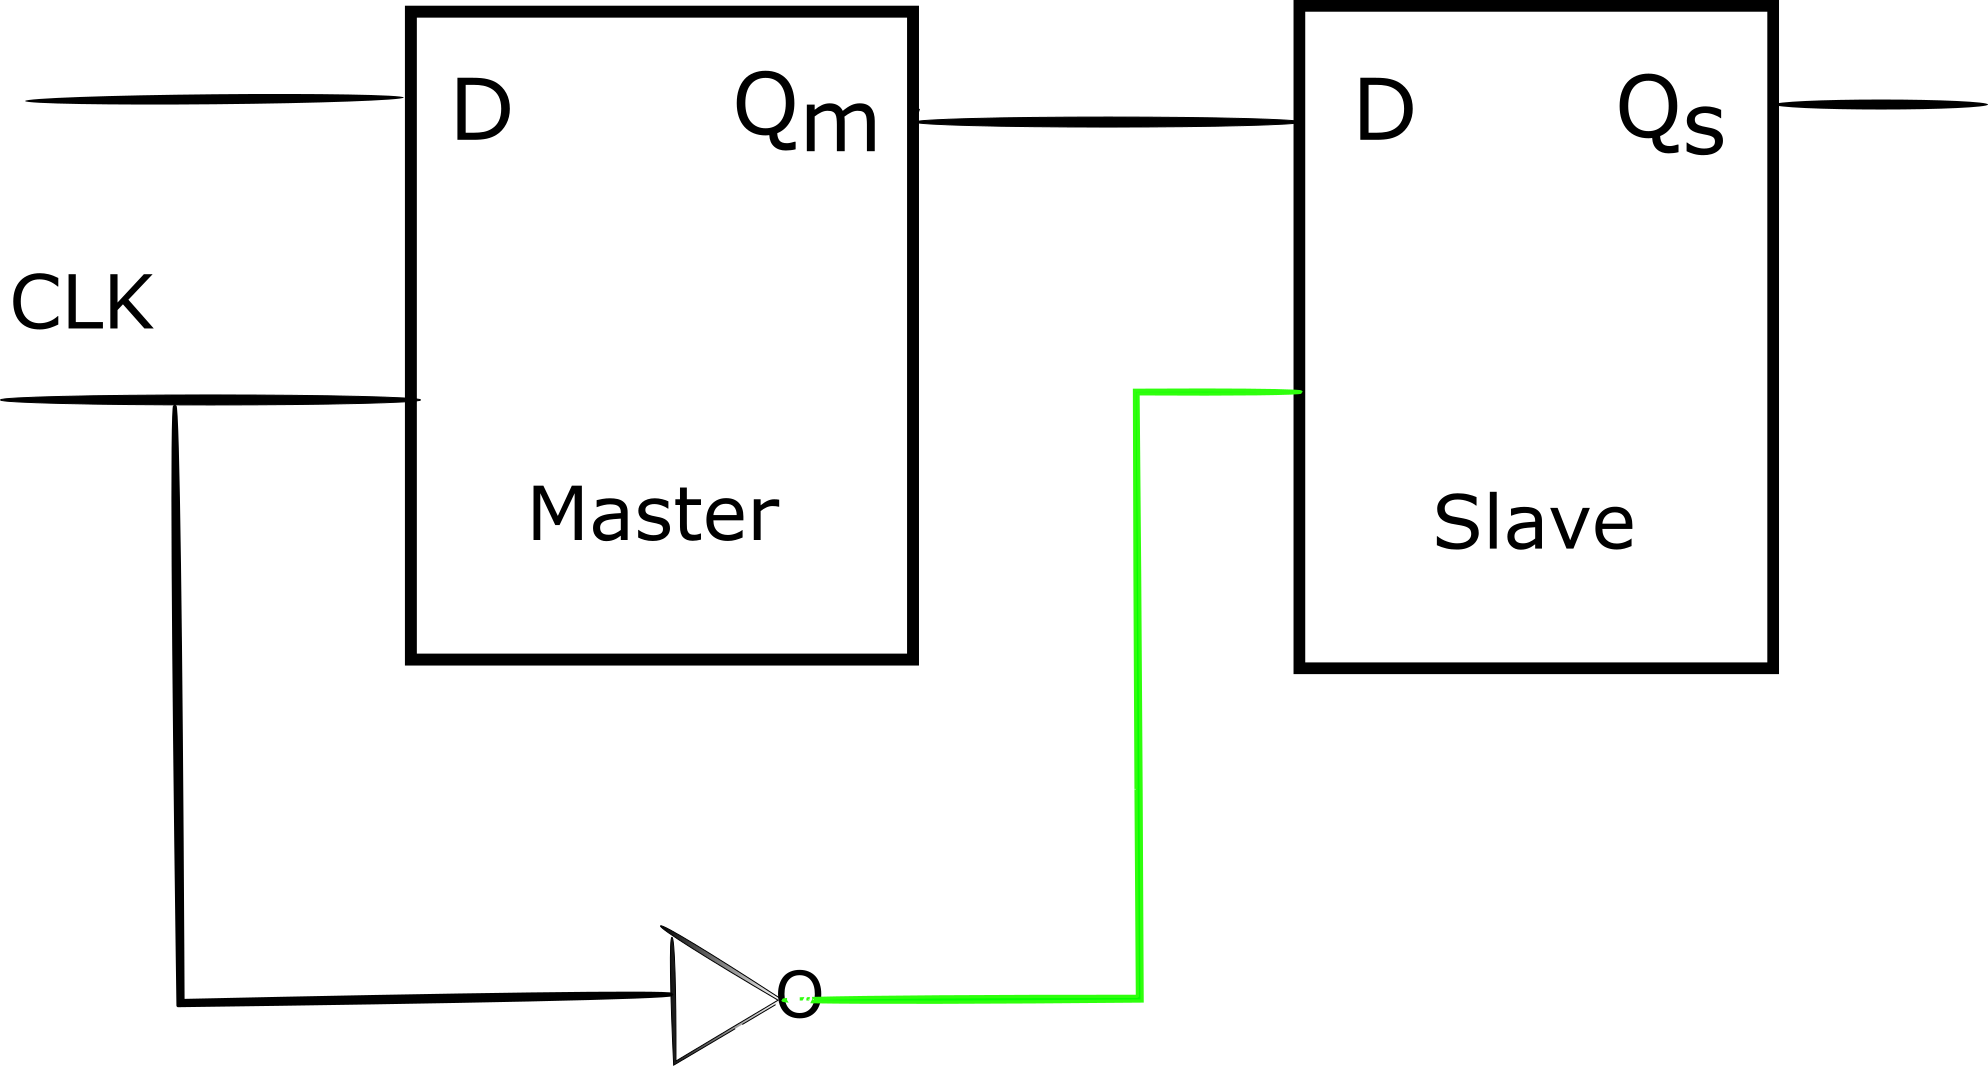
\includegraphics[width=.7\textwidth,height=100px]{name/path2.png}
\end{figure}
\begin{figure}[h]
    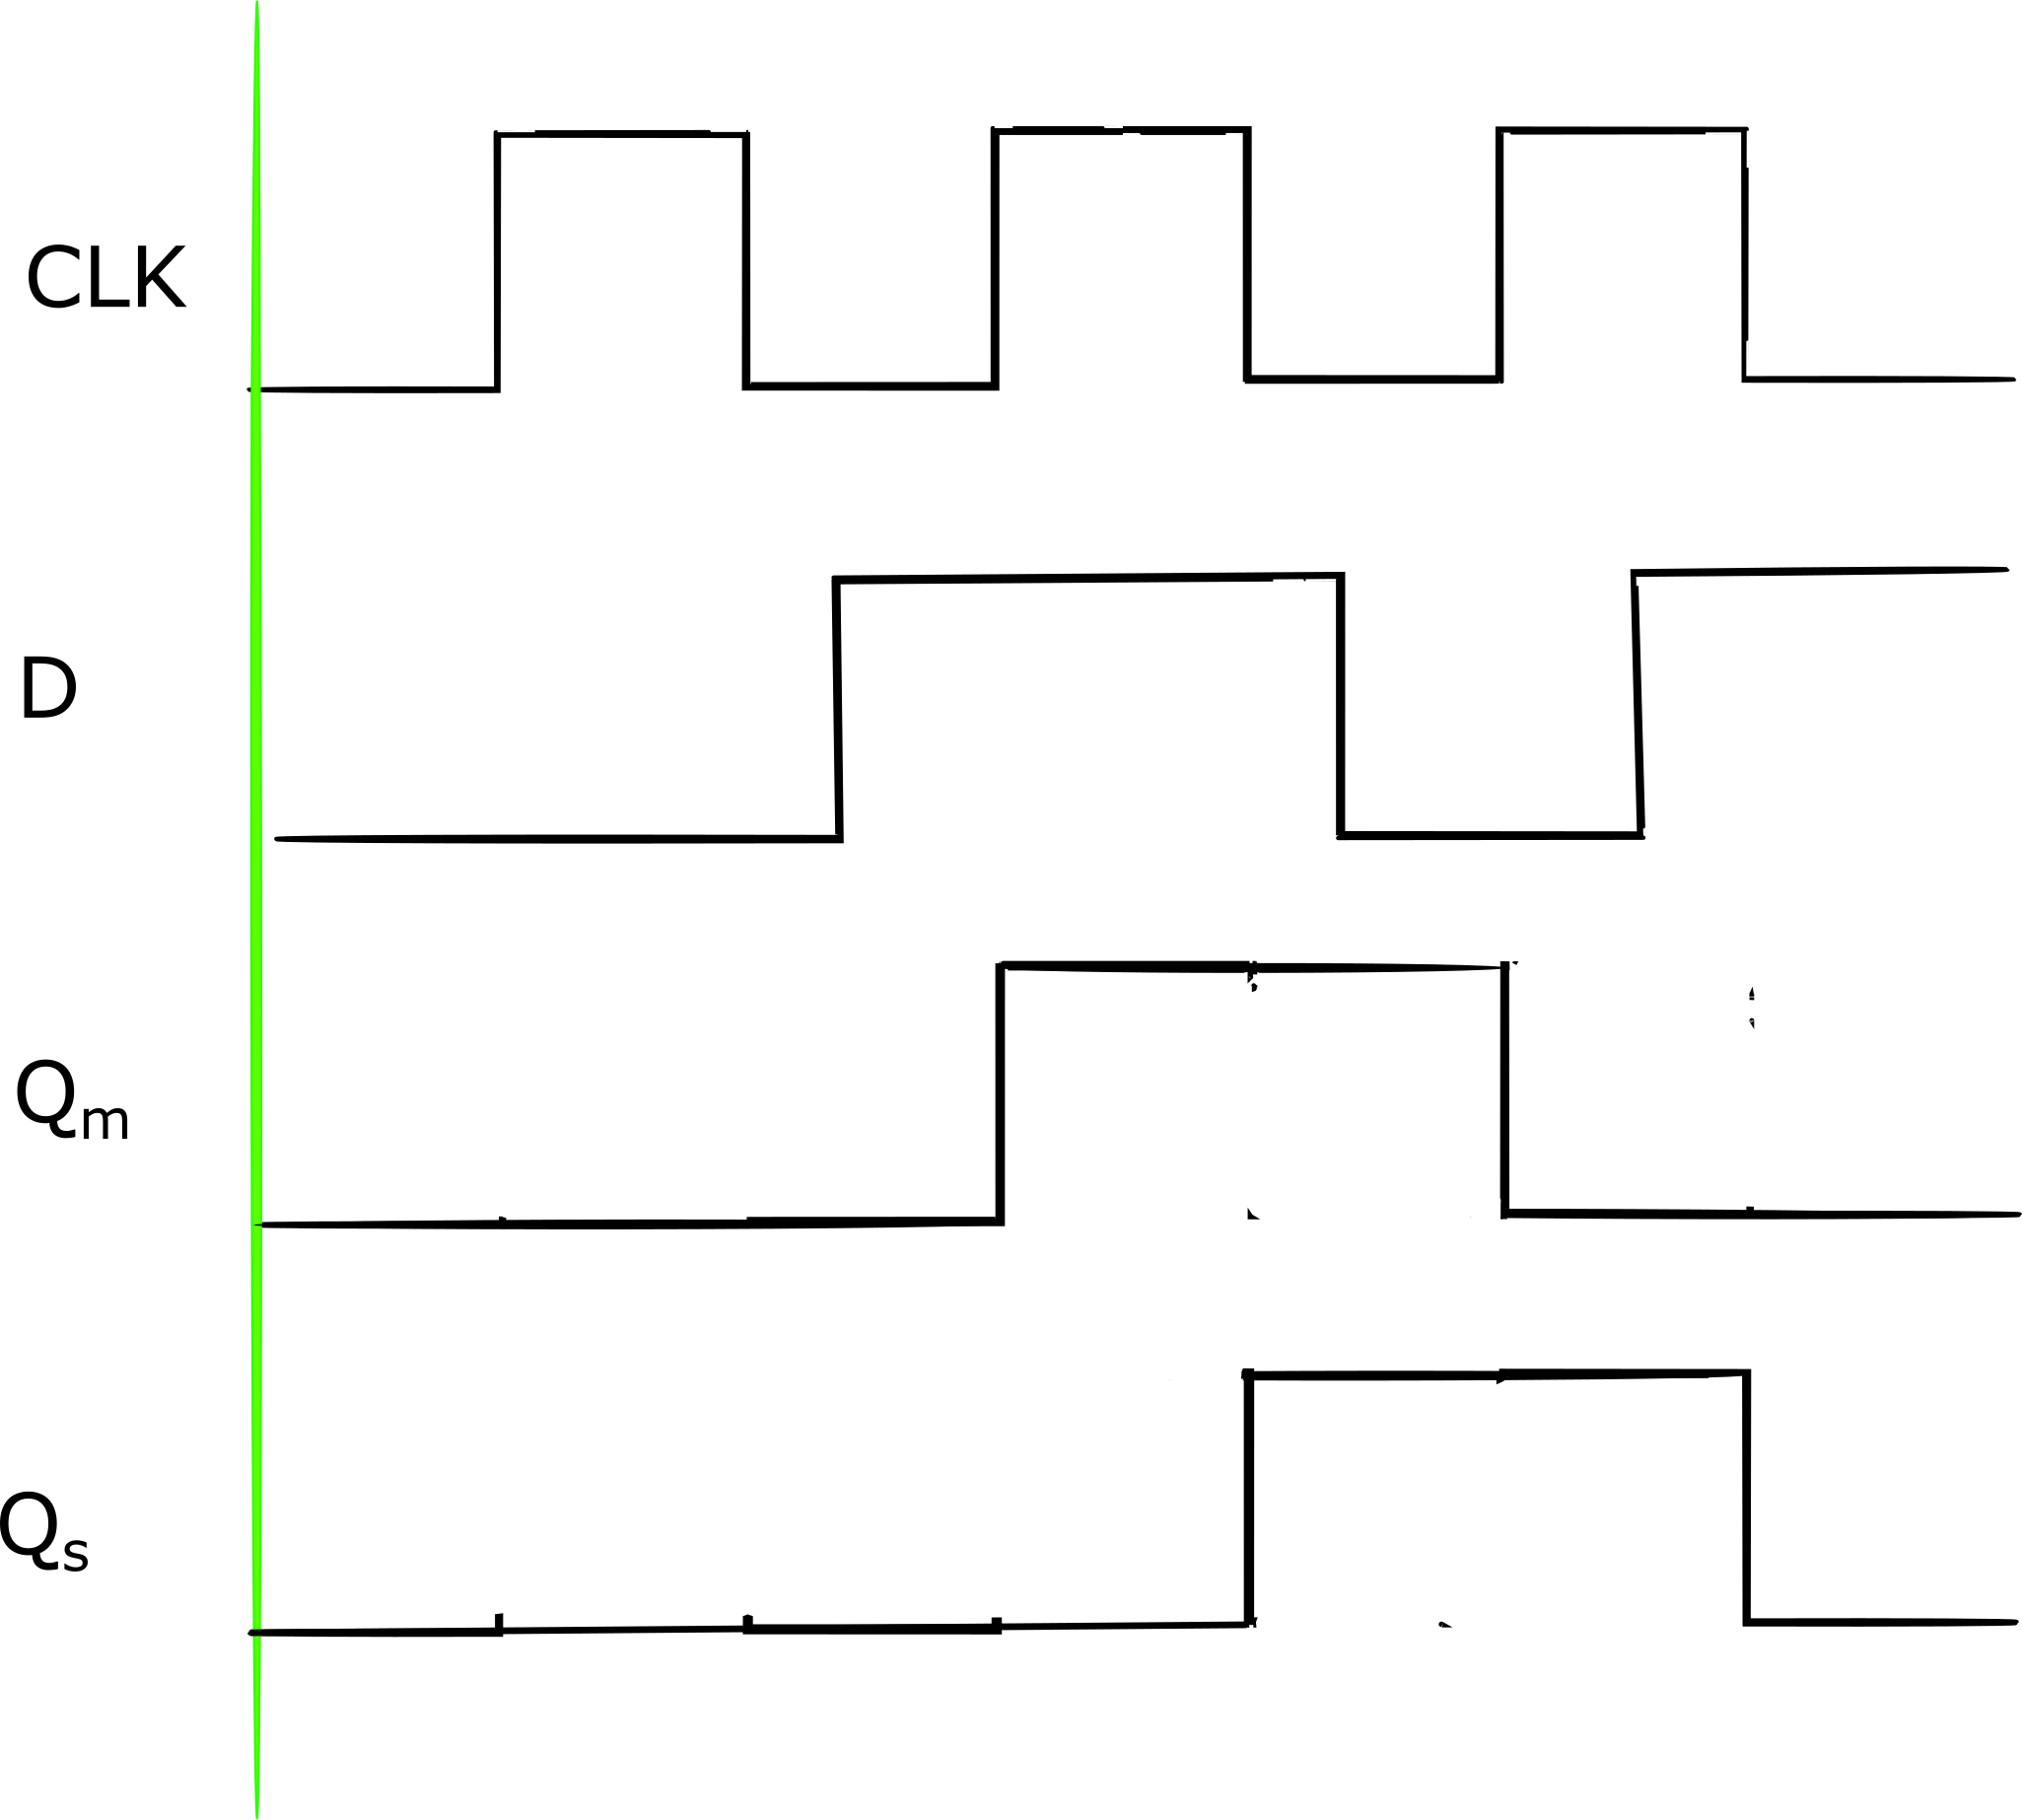
\includegraphics[width=.7\textwidth,height=100px]{name/clk0.png}
\end{figure}
\end{frame}


\begin{frame}
\frametitle{Simulation of Master Slave D flip flop}
\begin{figure}[h]
    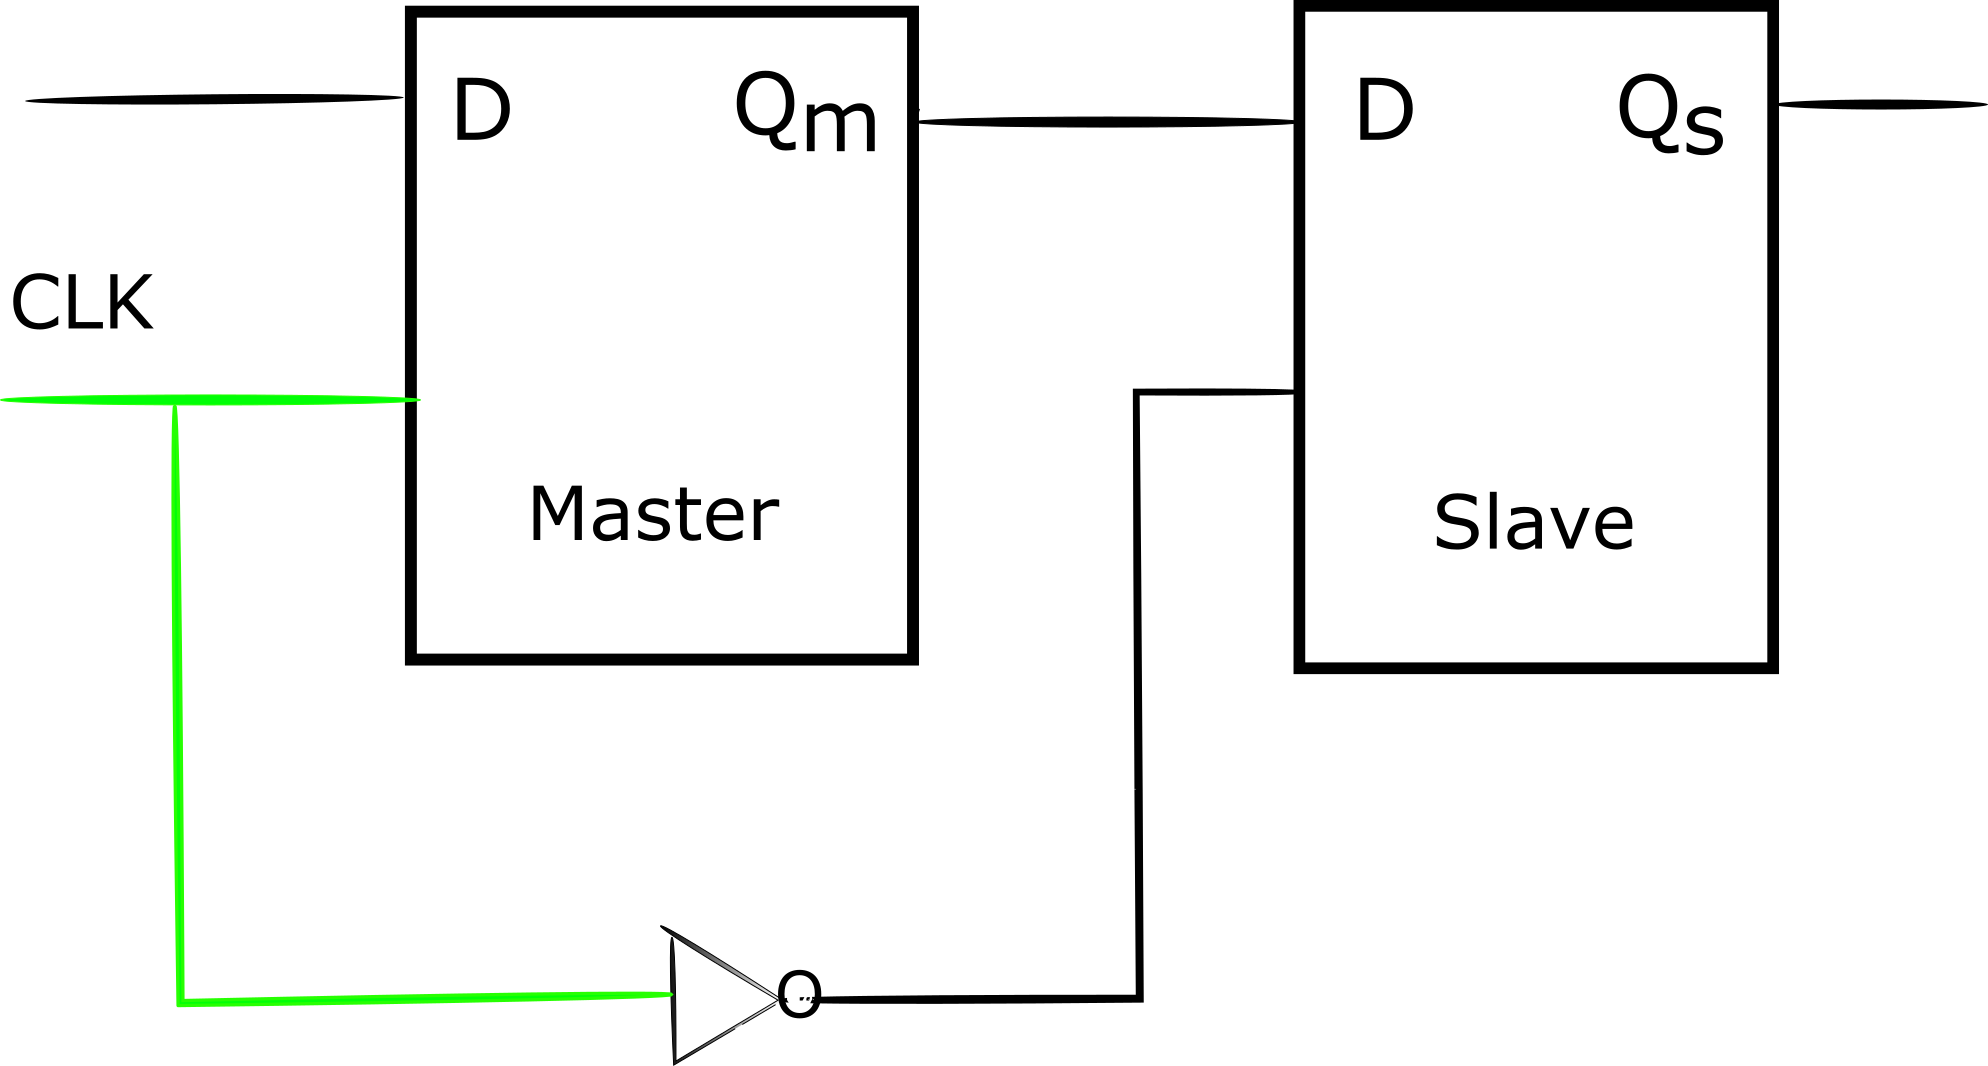
\includegraphics[width=.7\textwidth,height=100px]{name/path3.png}
\end{figure}
\begin{figure}[h]
    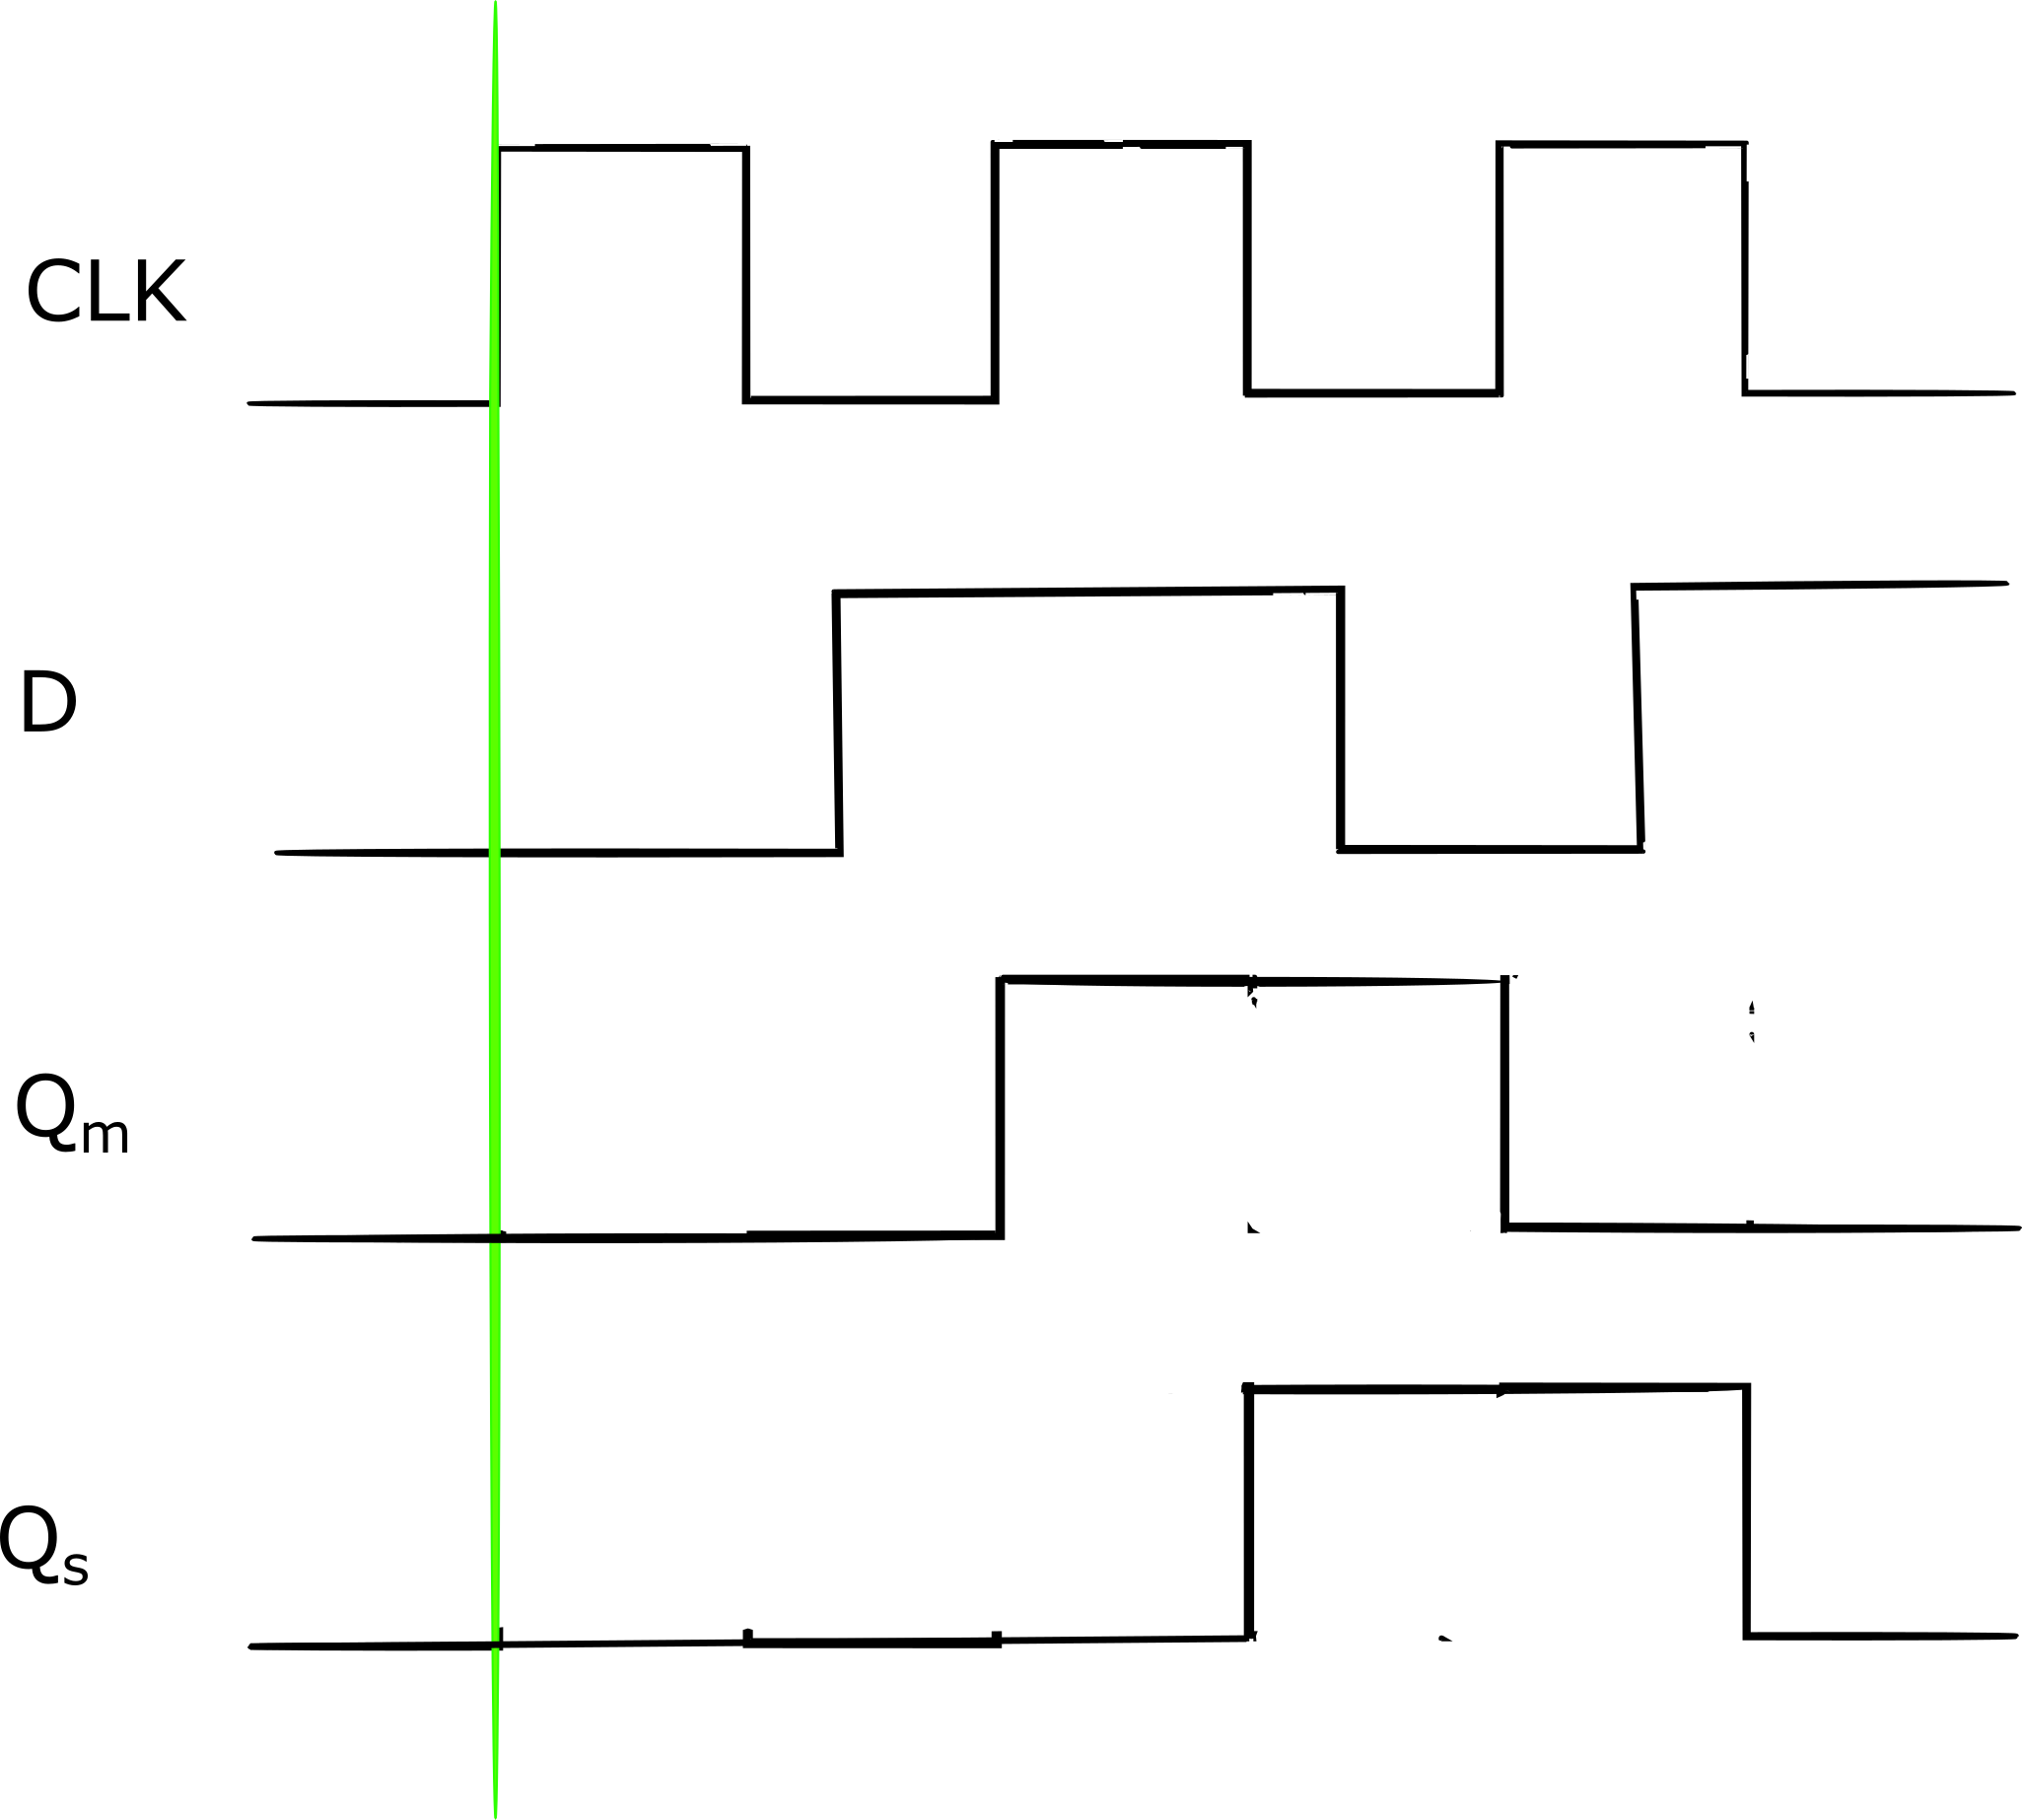
\includegraphics[width=.7\textwidth,height=100px]{name/clk1.png}
\end{figure}
\end{frame}

\begin{frame}
\frametitle{Simulation of Master Slave D flip flop}
\begin{figure}[h]
    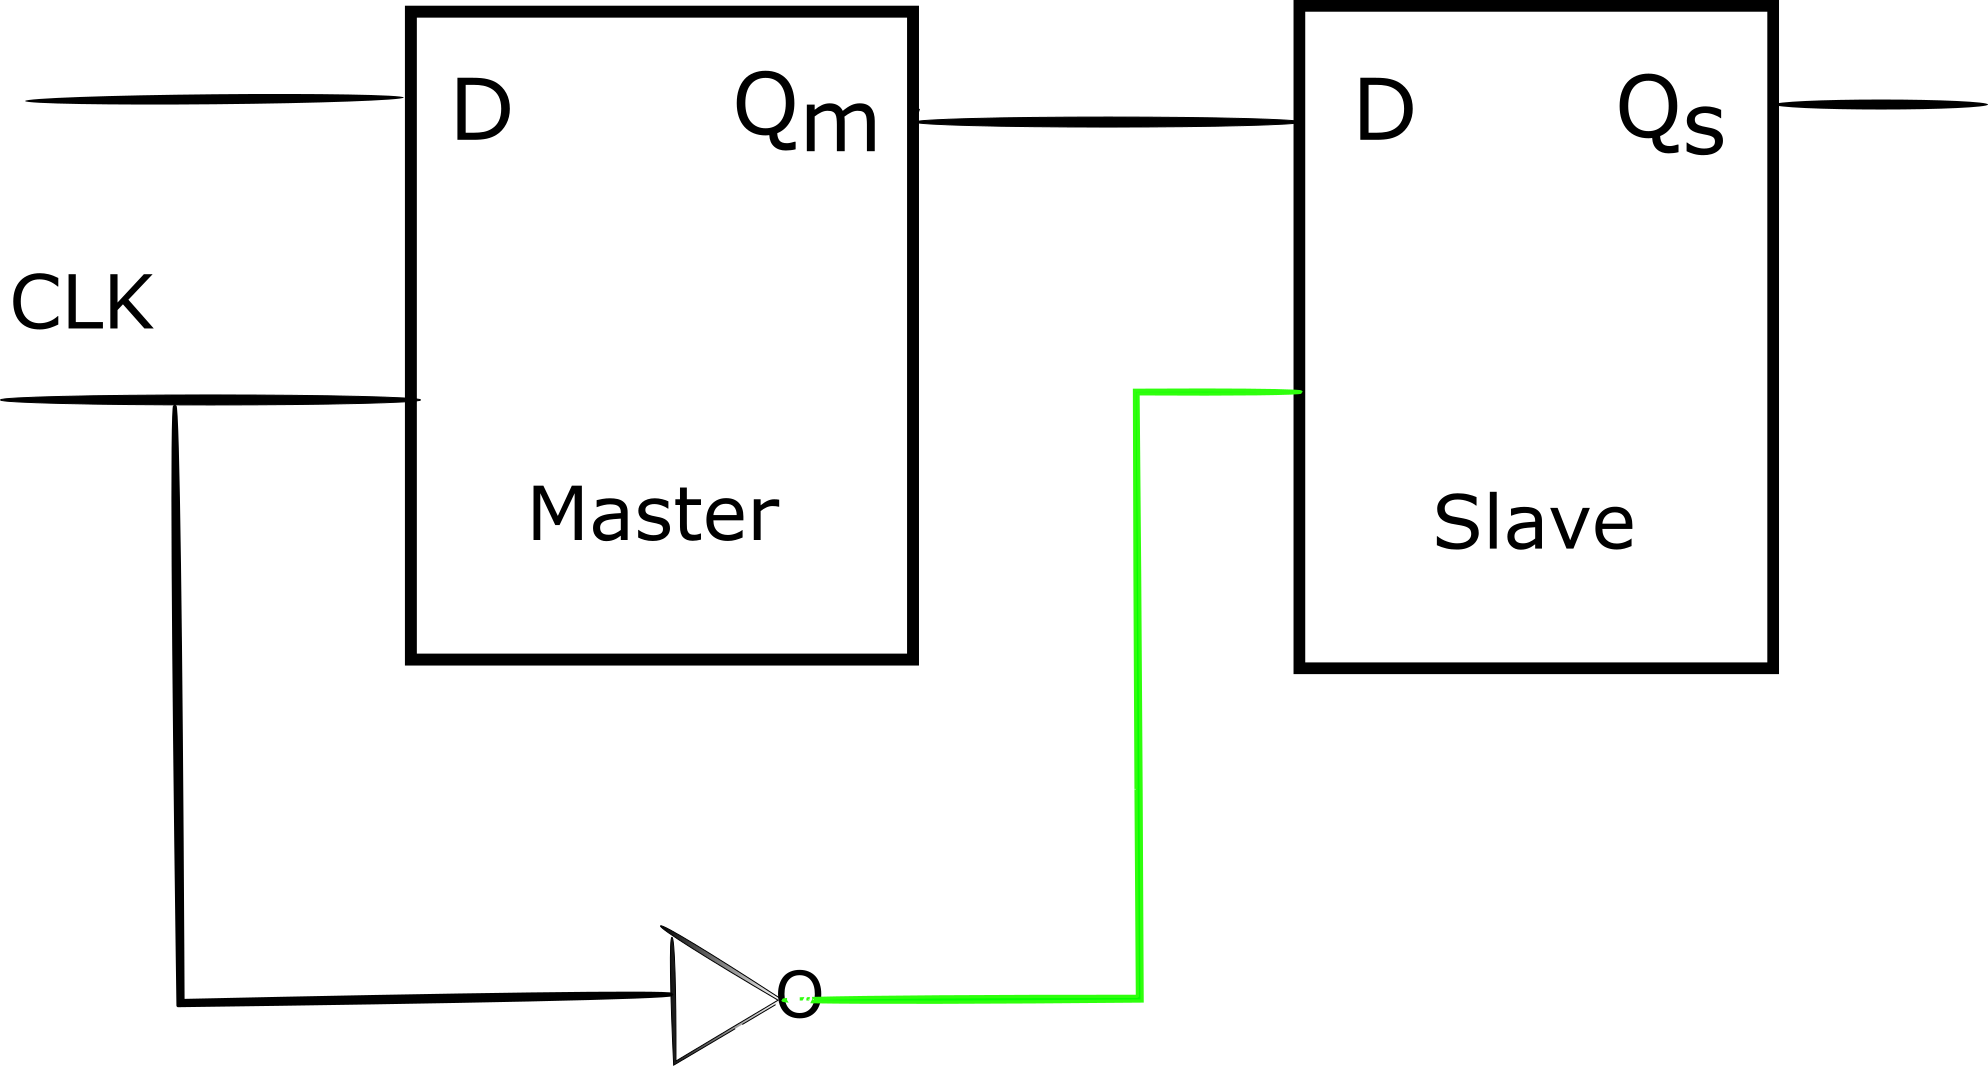
\includegraphics[width=.7\textwidth,height=100px]{name/path2.png}
\end{figure}
\begin{figure}[h]
    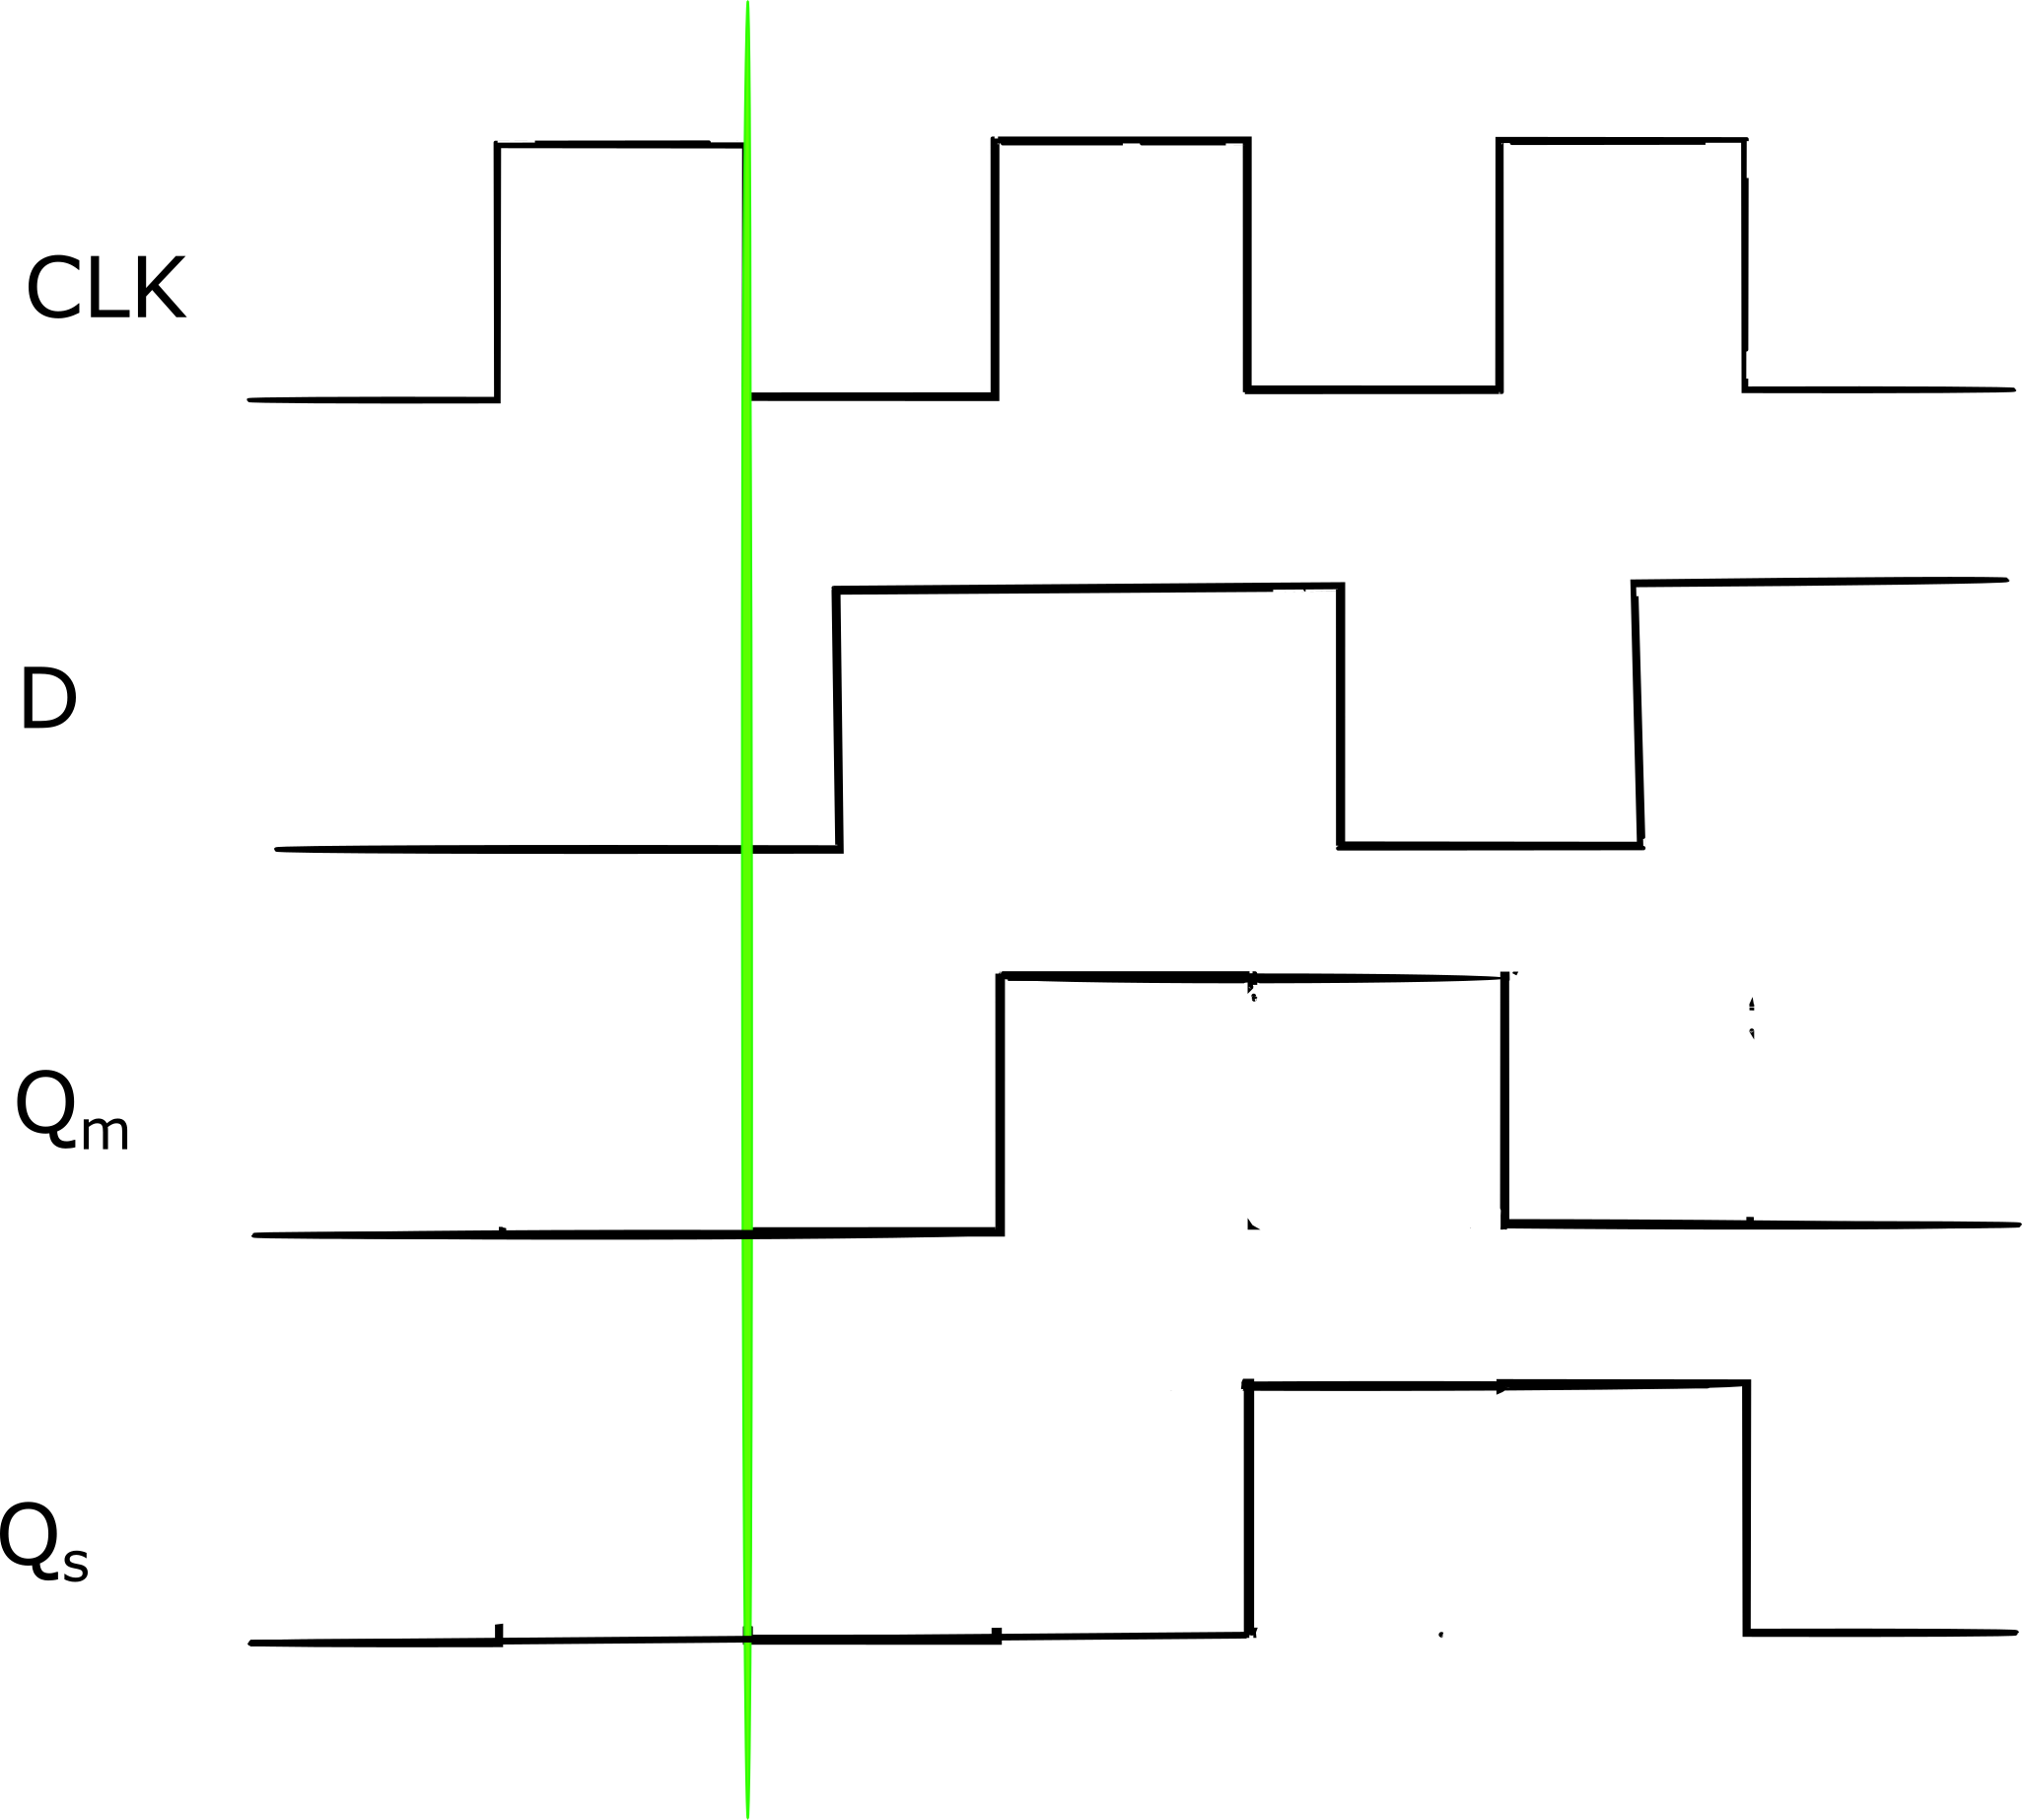
\includegraphics[width=.7\textwidth,height=100px]{name/clk2.png}
\end{figure}
\end{frame}

\begin{frame}
\frametitle{Simulation of Master Slave D flip flop}
\begin{figure}[h]
    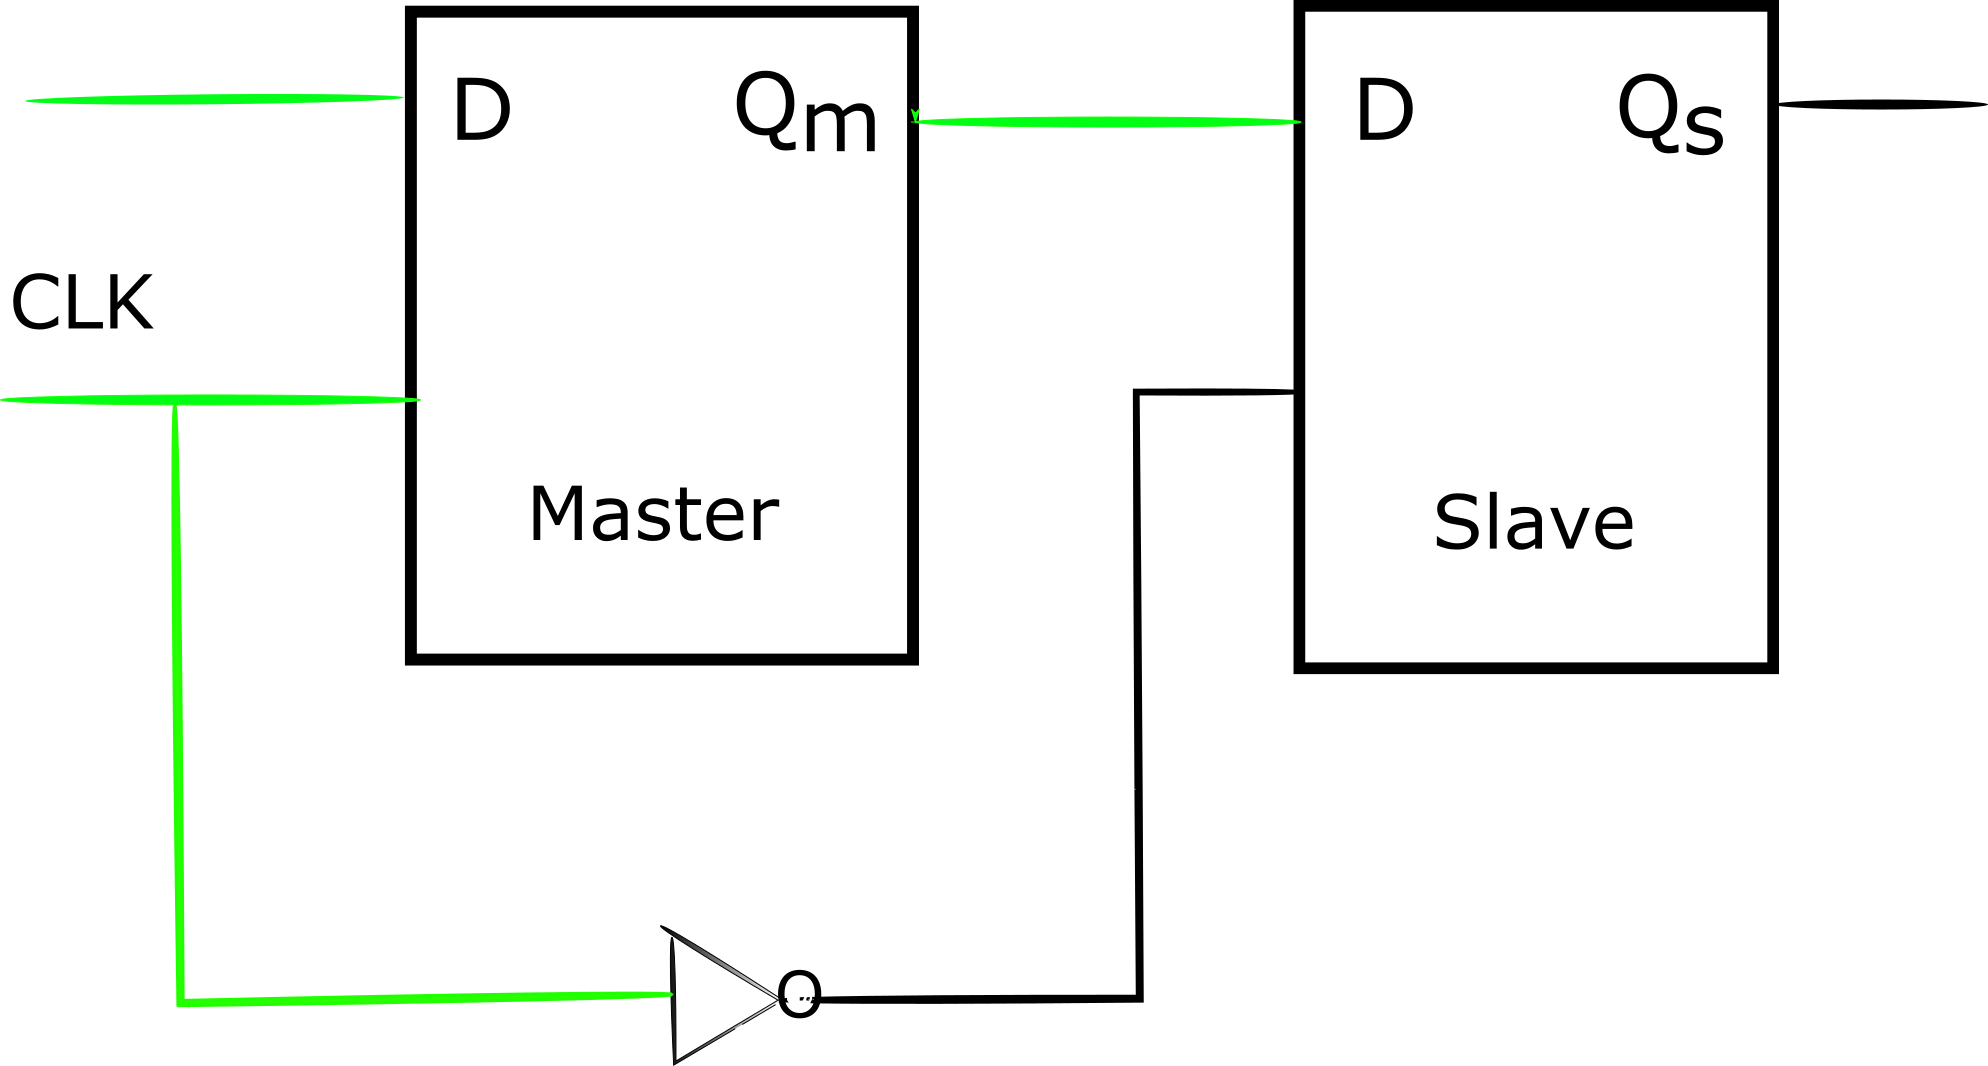
\includegraphics[width=.7\textwidth,height=100px]{name/path4.png}
\end{figure}
\begin{figure}[h]
    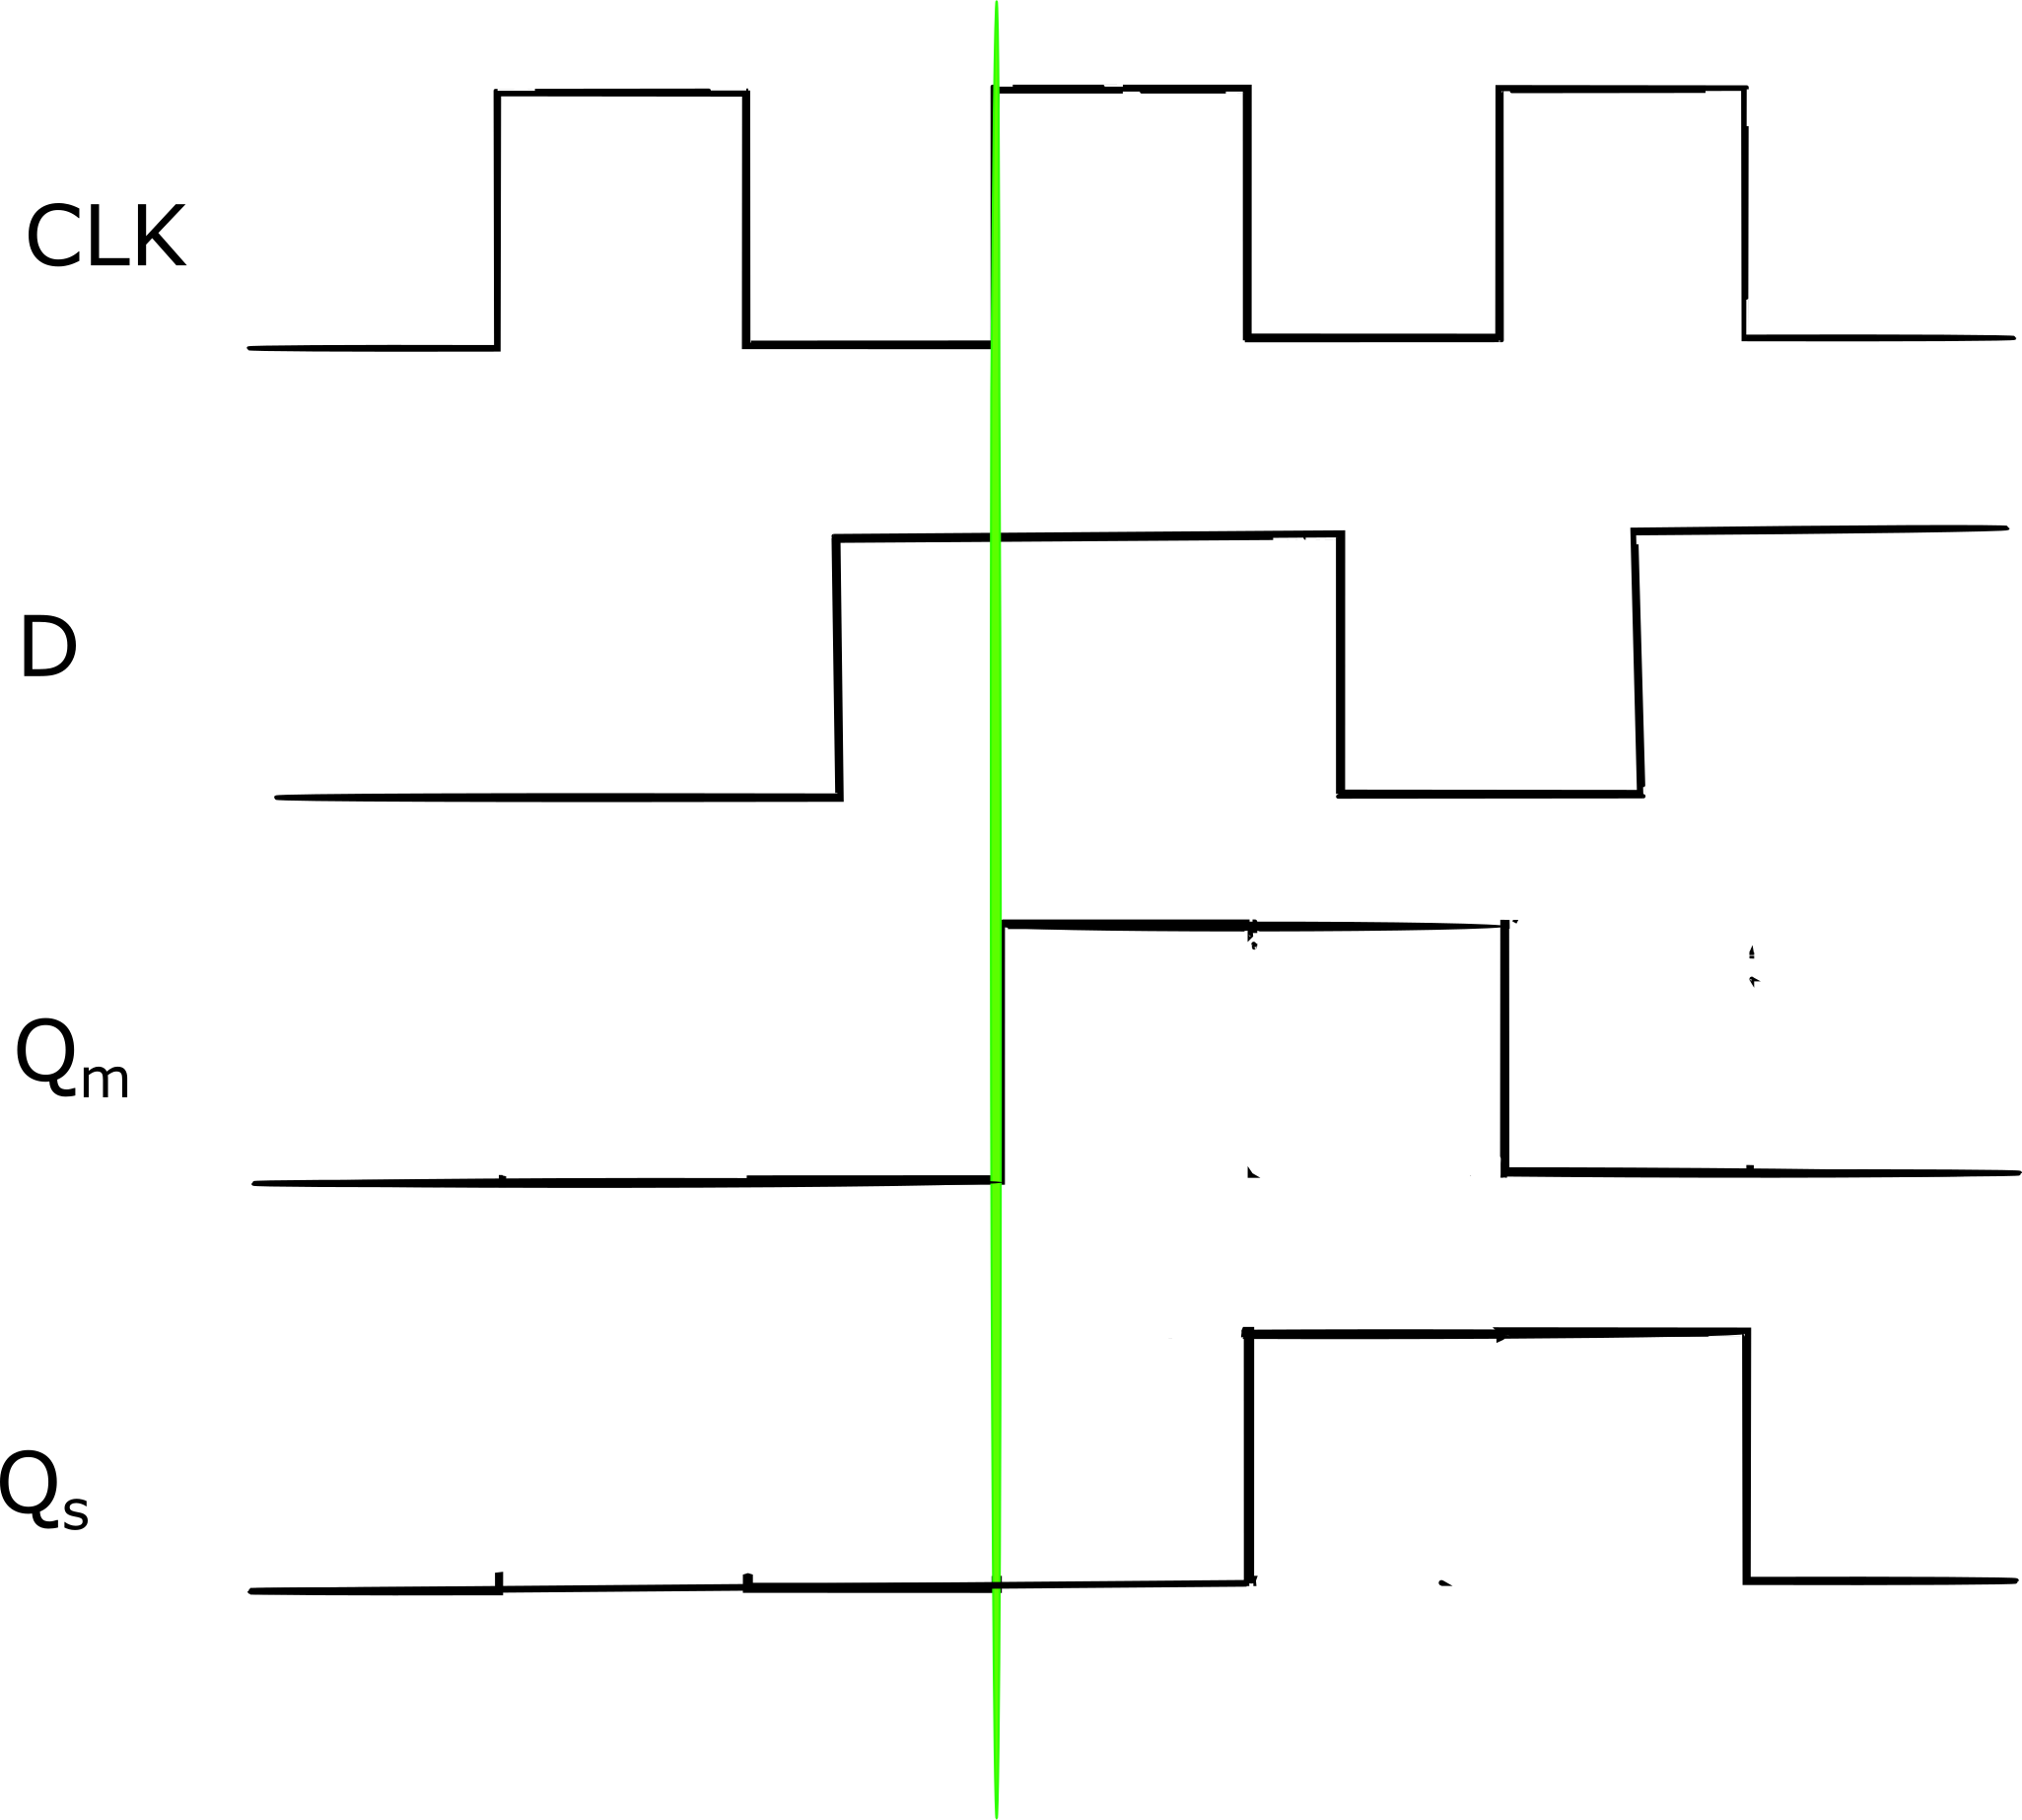
\includegraphics[width=.7\textwidth,height=100px]{name/clk4.png}
\end{figure}
\end{frame}

\begin{frame}
\frametitle{Simulation of Master Slave D flip flop}
\begin{figure}[h]
    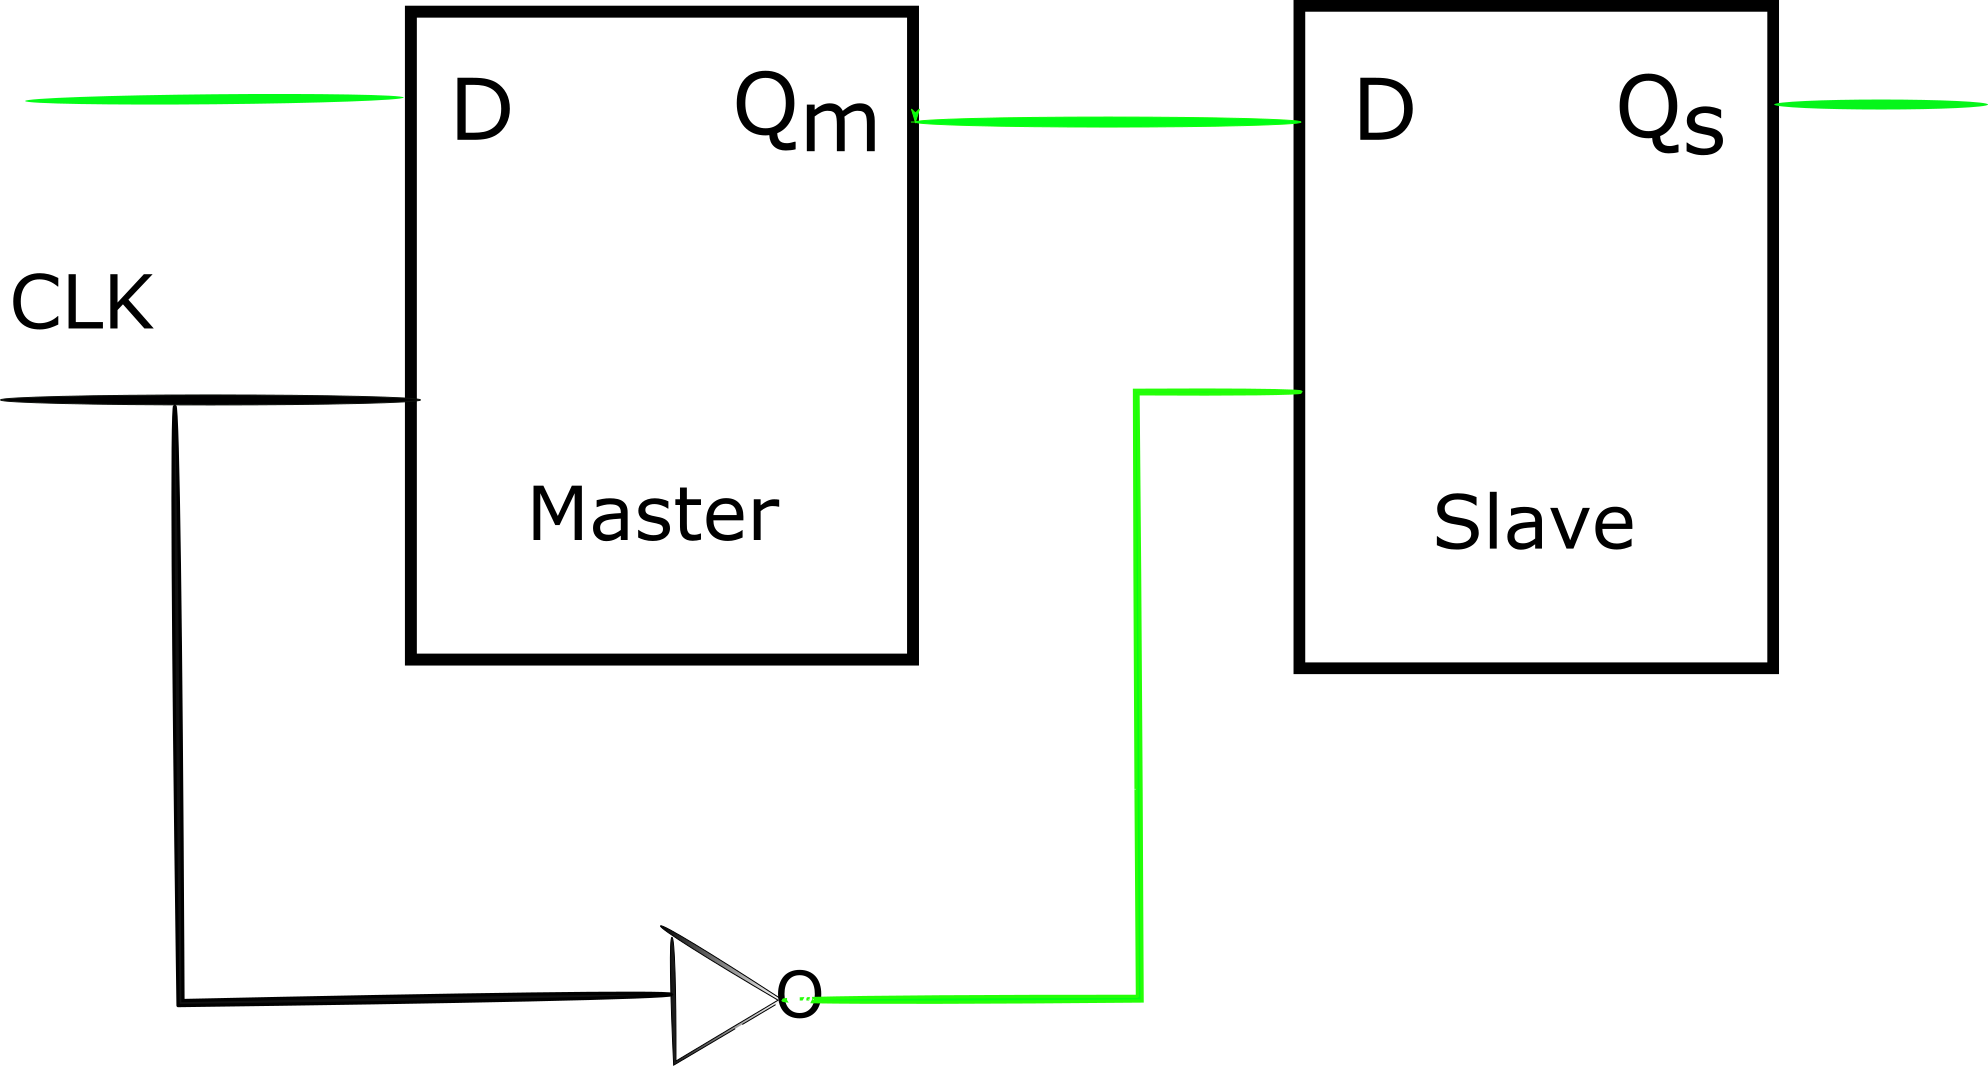
\includegraphics[width=.7\textwidth,height=100px]{name/path5.png}
\end{figure}
\begin{figure}[h]
    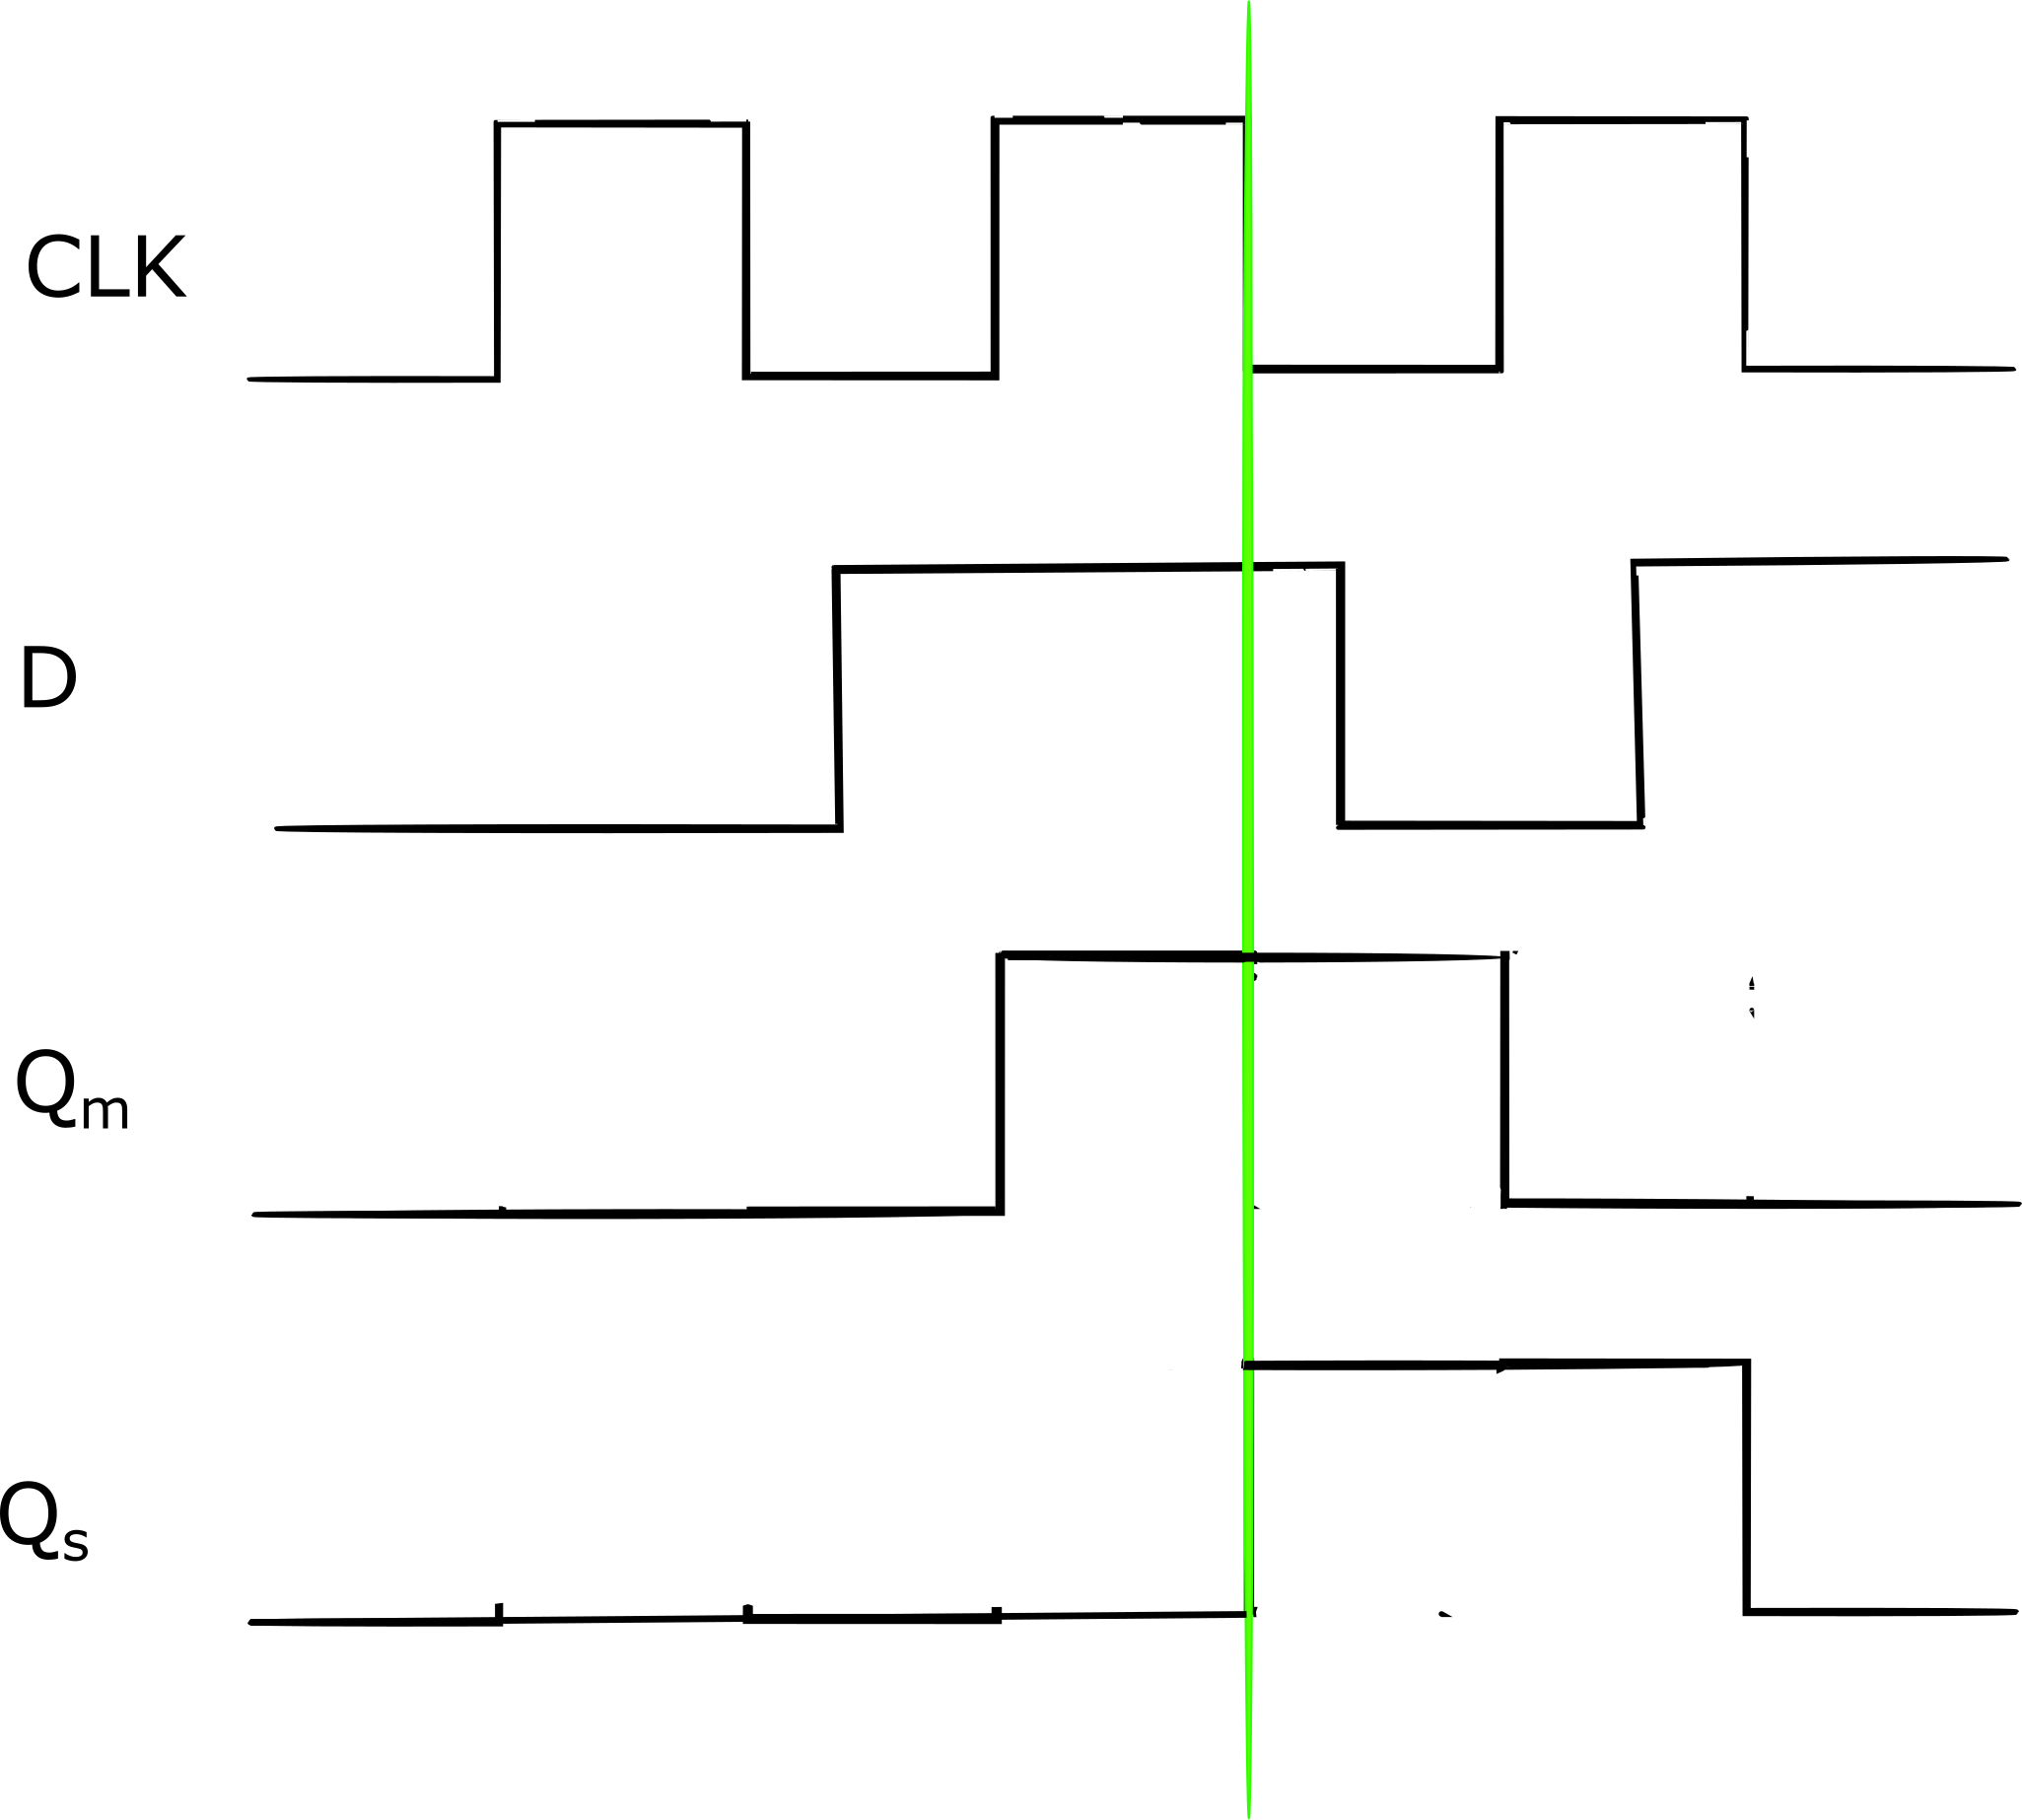
\includegraphics[width=.7\textwidth,height=100px]{name/clk5.png}
\end{figure}
\end{frame}

\begin{frame}
\frametitle{Simulation of Master Slave D flip flop}
\begin{figure}[h]
    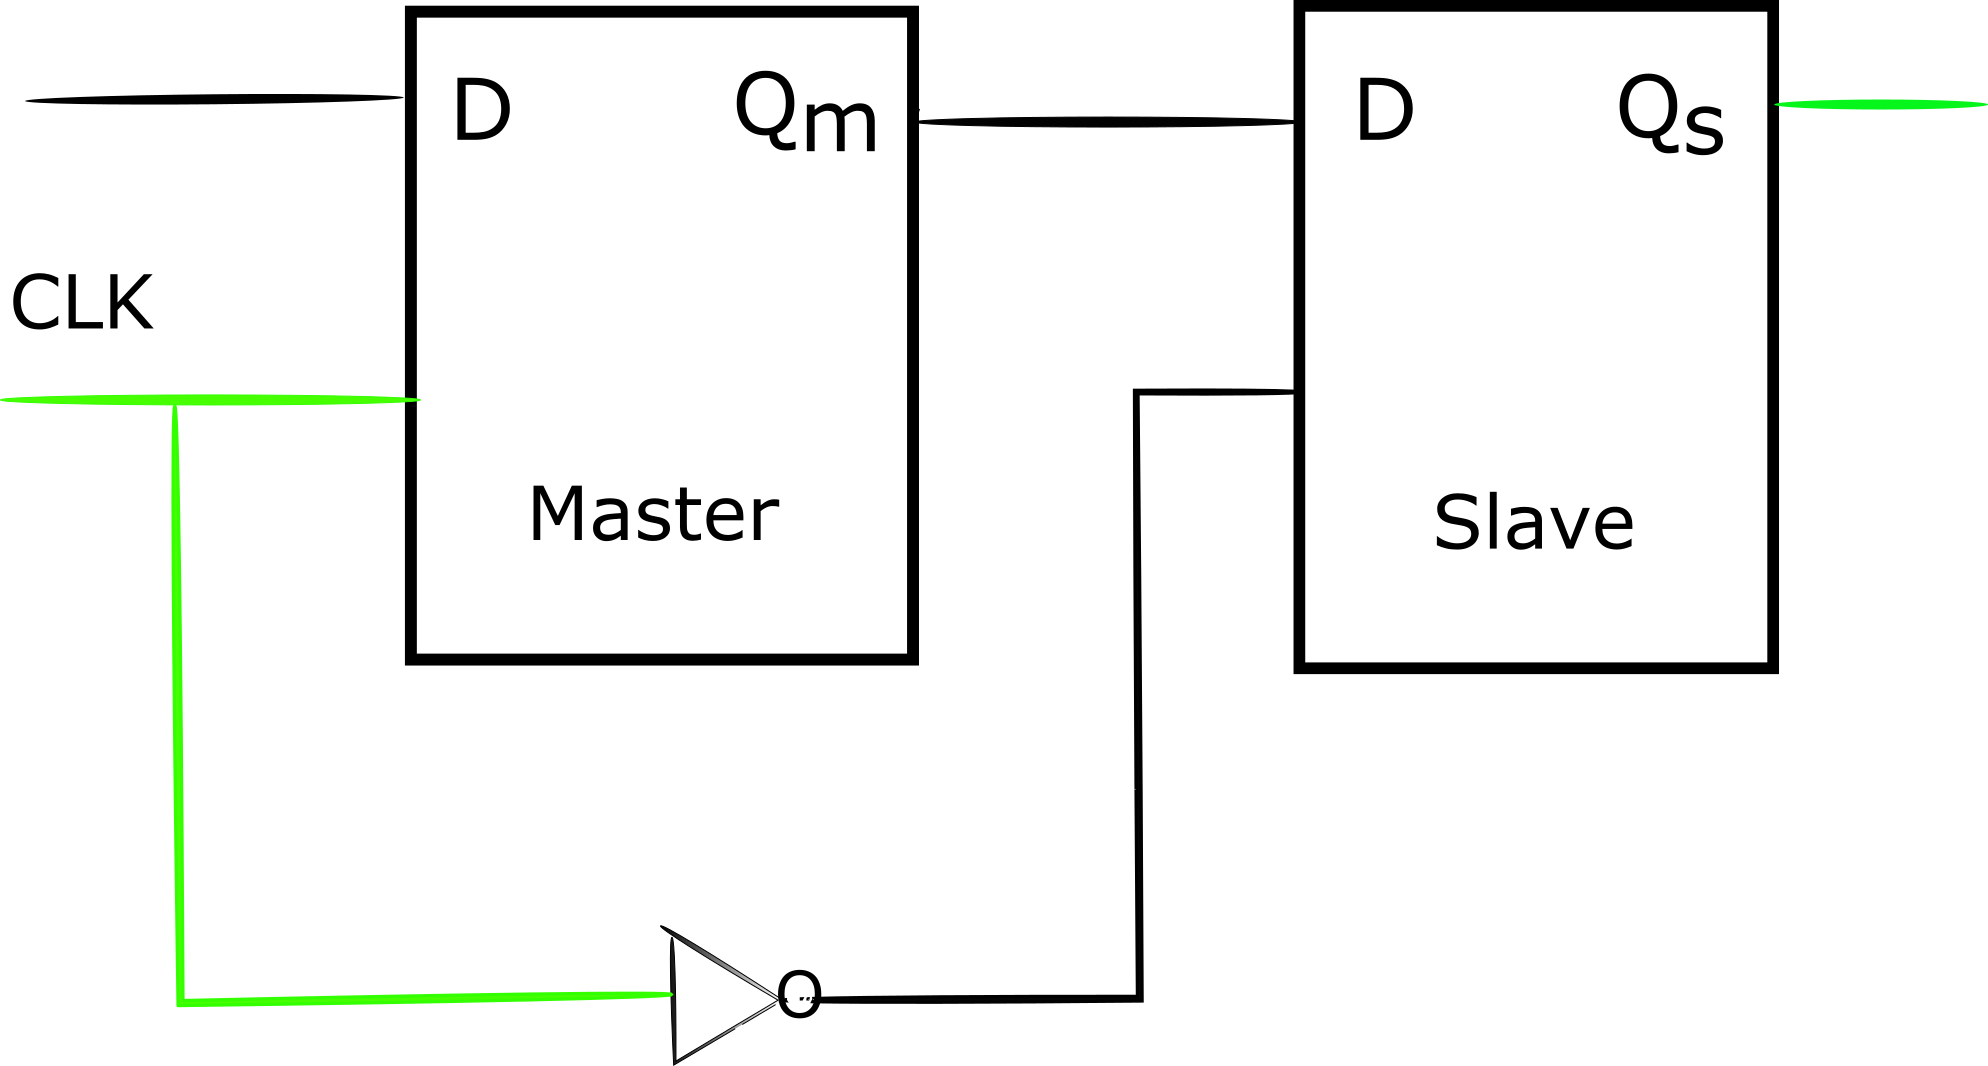
\includegraphics[width=.7\textwidth,height=100px]{name/path6.png}
\end{figure}
\begin{figure}[h]
    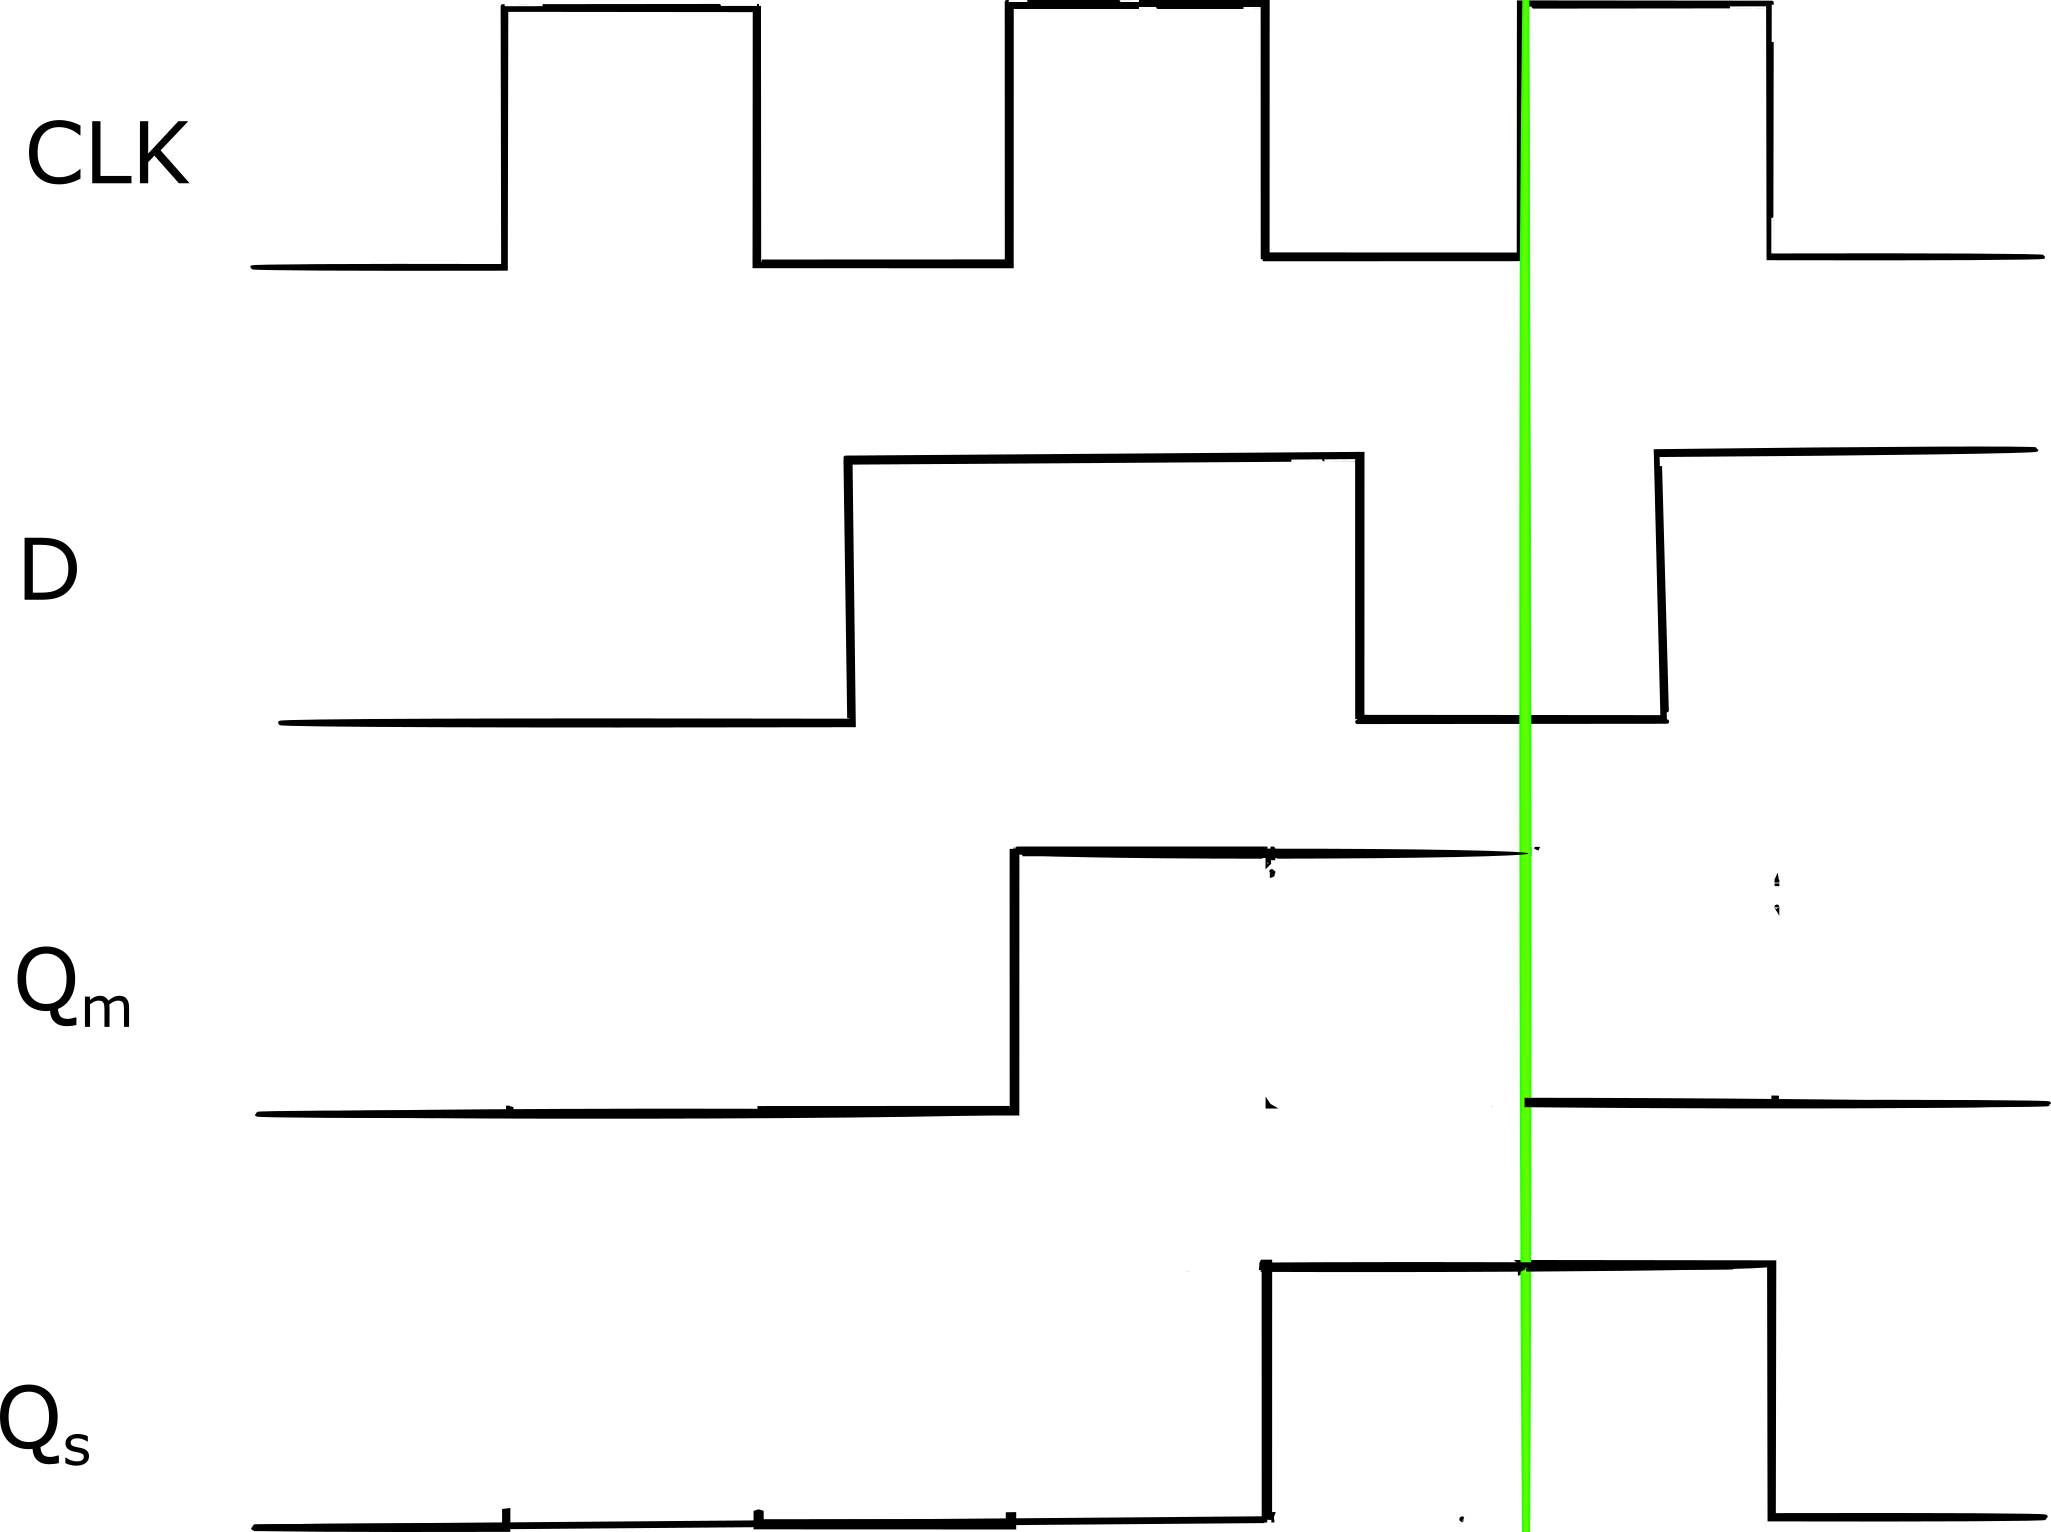
\includegraphics[width=.7\textwidth,height=100px]{name/clk6.png}
\end{figure}
\end{frame}

\begin{frame}
\frametitle{Simulation of Master Slave D flip flop}
\begin{figure}[h]
    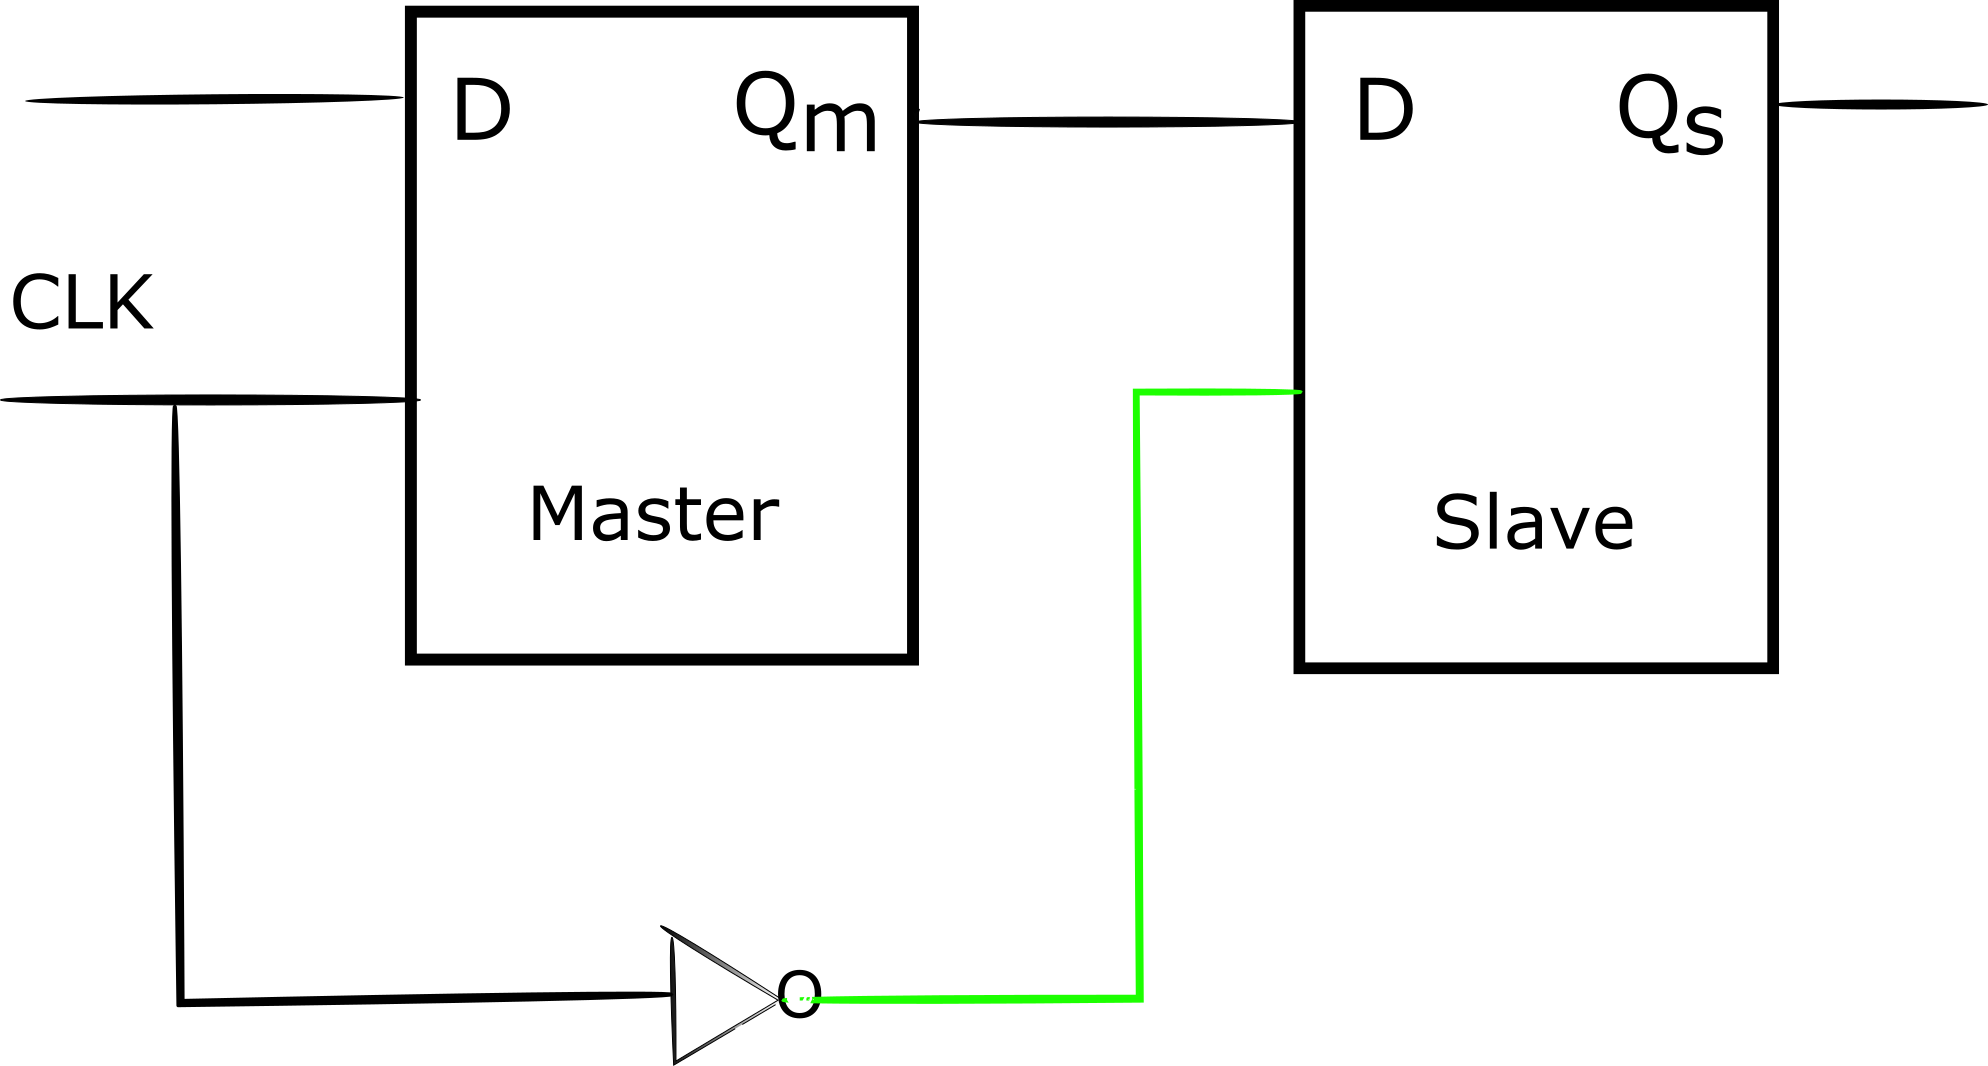
\includegraphics[width=.7\textwidth,height=100px]{name/path7.png}
\end{figure}
\begin{figure}[h]
    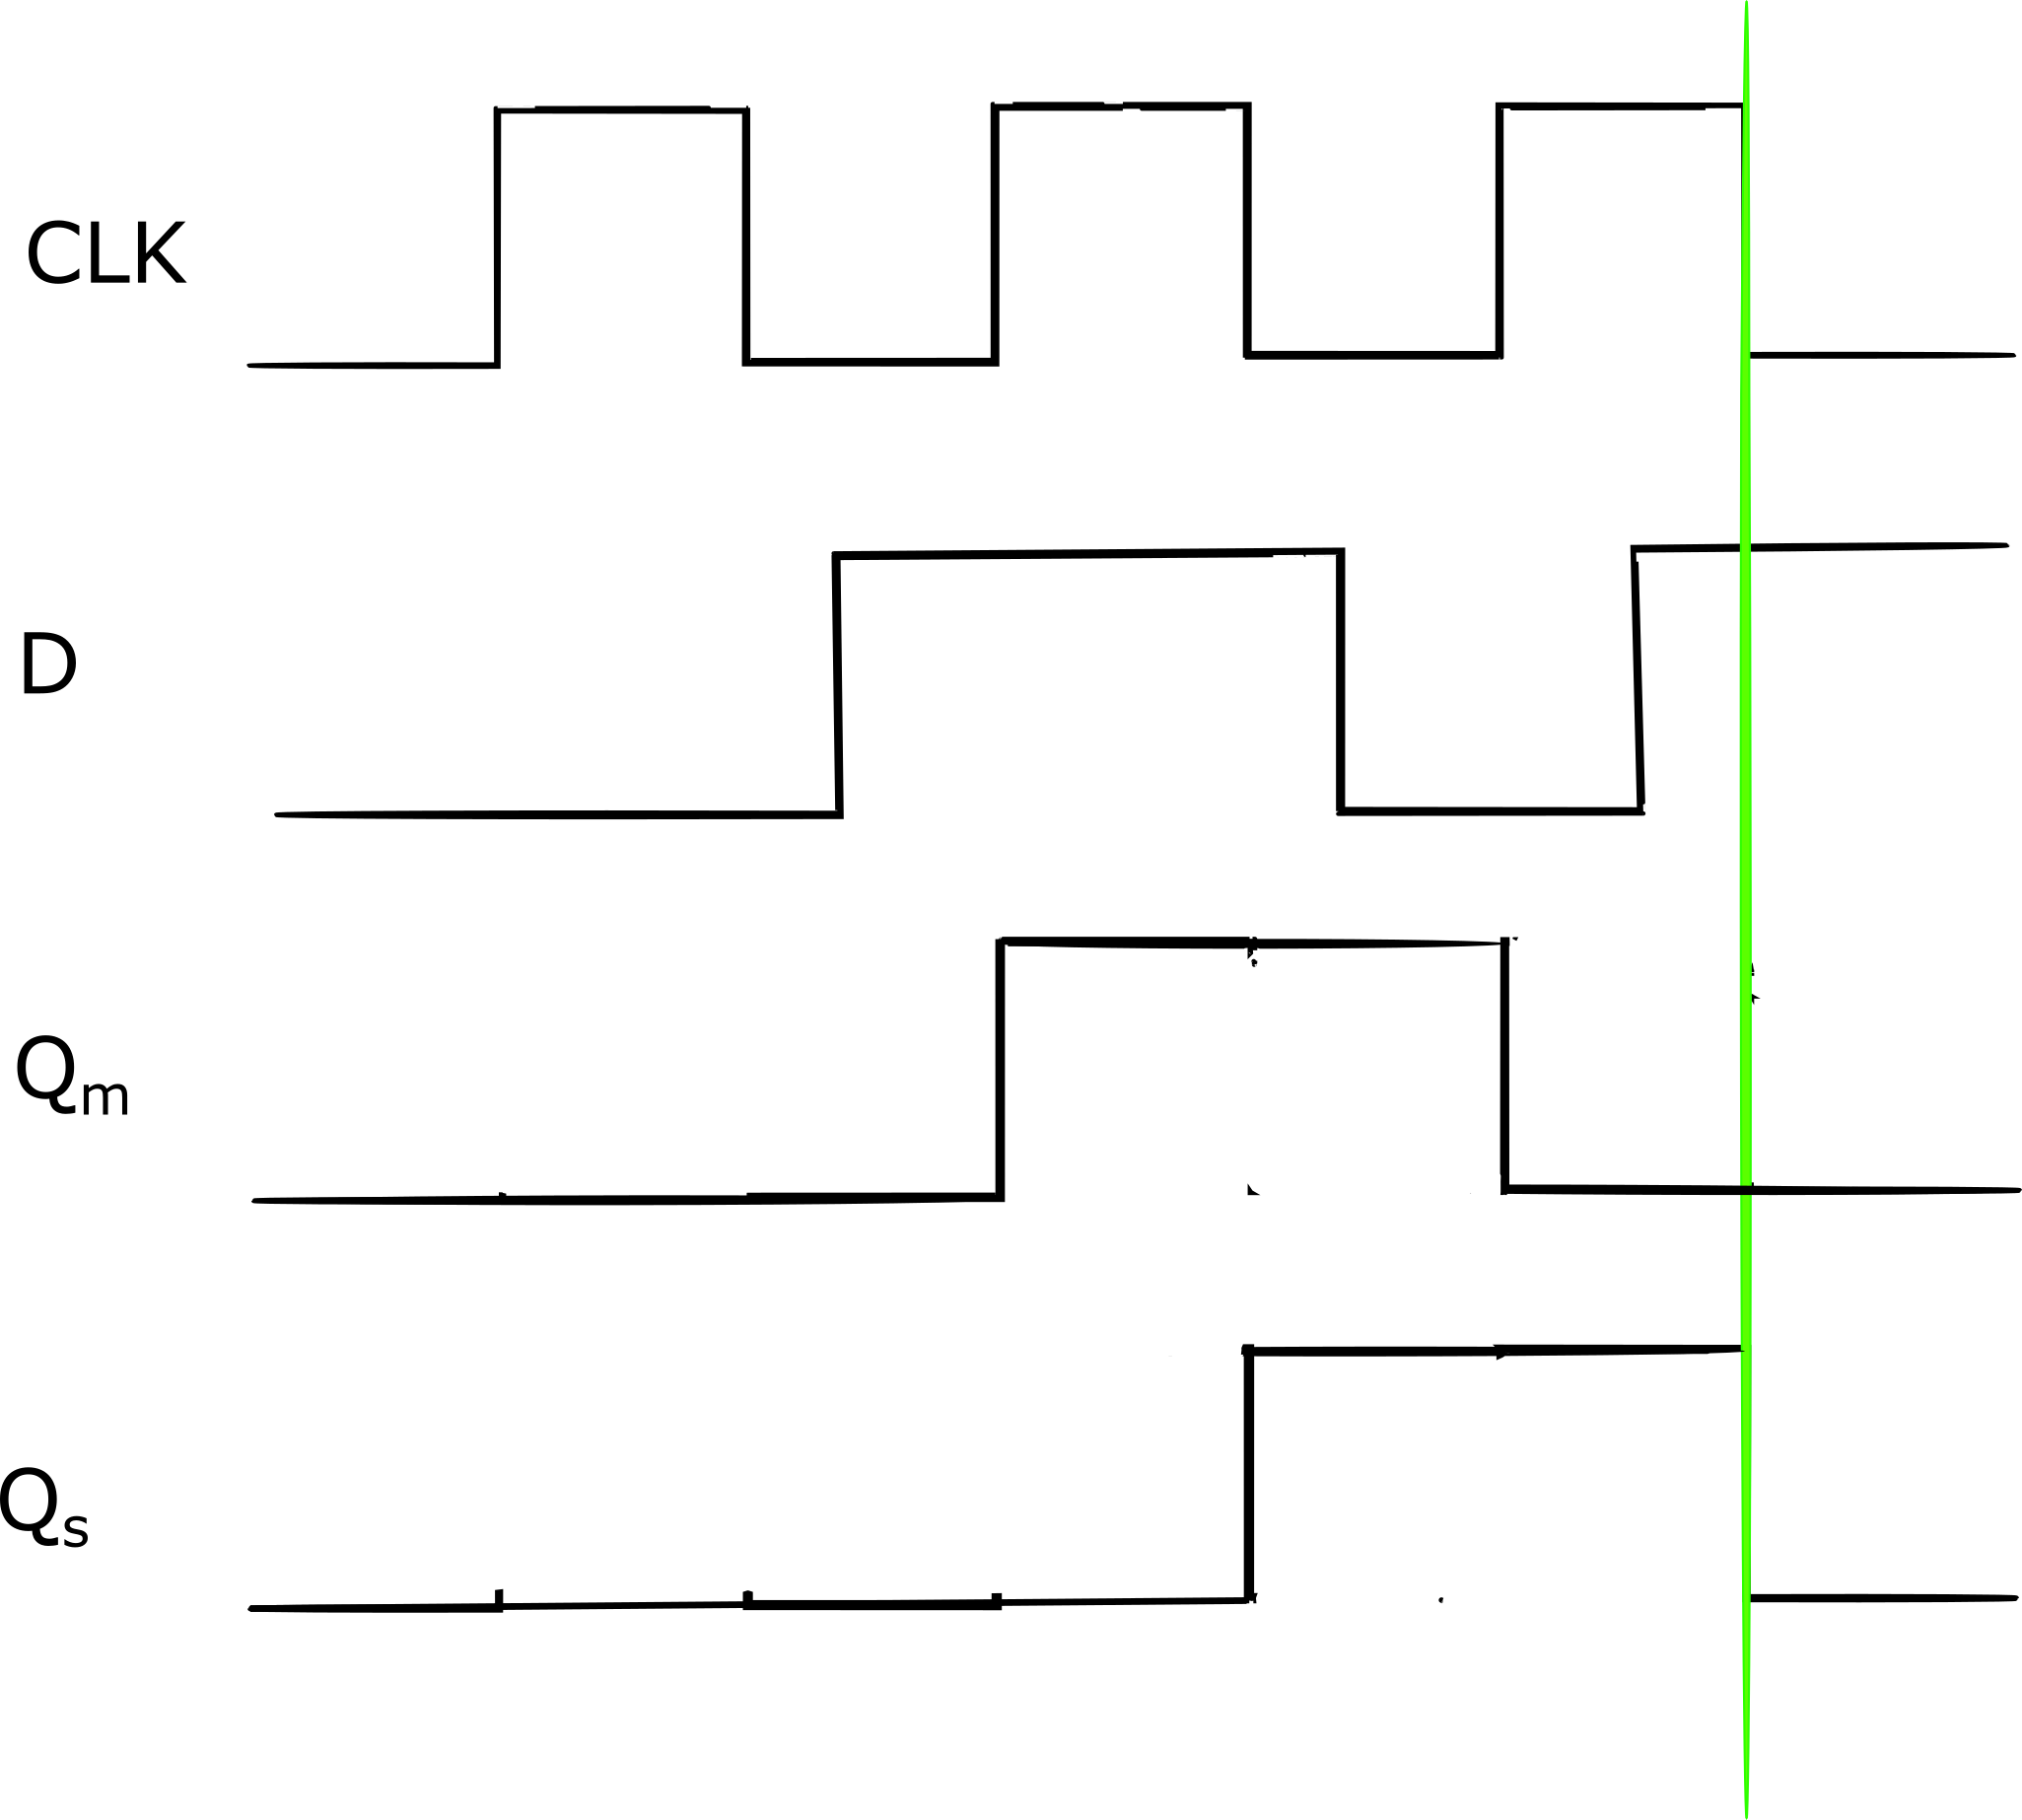
\includegraphics[width=.7\textwidth,height=100px]{name/clk7.png}
\end{figure}
\end{frame}



\begin{frame}
    
    
    \alert{What will be the timing diagram for negative edge triggered Master Slave flip flop?}\pause
    \begin{figure}[H]
        \centering
        
        %\def\svgscale{1}
        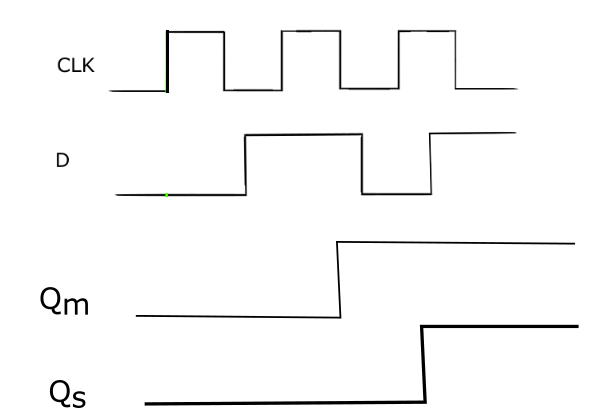
\includegraphics[scale=.5]{name/path2100.png}
        
        
        %\caption{T type Flip Flop}
        \label{fig:my_label}
    \end{figure}
    
\end{frame}

\begin{frame}
    
    
    \begin{figure}[H]
        \centering
        
        %\def\svgscale{1}
        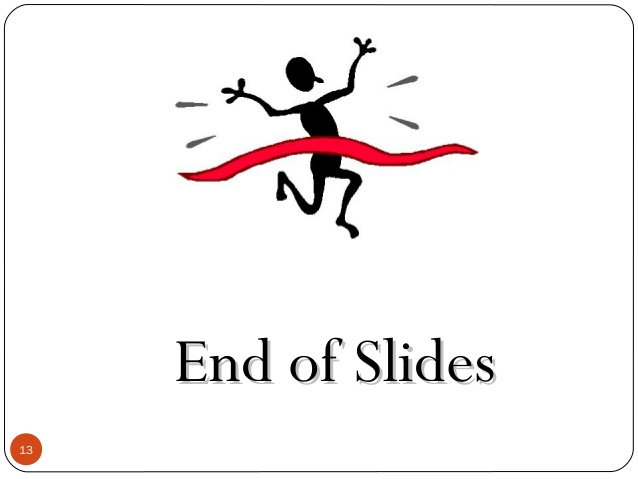
\includegraphics[scale=.35]{images/finite-automata-13-638.jpg}
        
        
        %\caption{T type Flip Flop}
        \label{fig:my_label}
    \end{figure}
    
\end{frame}



\end{document}
